\documentclass{Physics_H_Notes}
\usepackage{upgreek}
\usetikzlibrary{3d,calc,positioning, shapes.geometric,decorations.fractals,arrows,intersections,decorations.text,shapes}
\begin{document}
	
%\definecolor{softblue}{rgb}{0.92,0.95,0.99}
\thispagestyle{empty}
	\begin{tikzpicture}[remember picture,overlay,shorten >= -10pt]
		\fill[green!2!white] (current page.south west) rectangle (current page.north east);
		
		\coordinate (B1) at ([xshift=-8pt,yshift=-400pt]current page.north west);
		\coordinate (B2) at ([xshift=-8pt,yshift=-125pt]current page.north west);
		\coordinate (B3) at ([xshift=-50, yshift=-475pt]current page.north west);
		\coordinate (B4) at ([xshift=10pt,yshift=300pt]current page.south east);
		\coordinate (B5) at ([xshift=10pt,yshift=455pt]current page.south east);
		\coordinate (B6) at ([xshift=-300pt,yshift=-15pt]current page.south east);
		\coordinate (B7) at ([xshift=0pt,yshift=80pt]current page.south east);
		
		\begin{scope}[decoration=Koch snowflake]
			\draw (B3)  ++(43:7)coordinate(C3)  ++(123:7)coordinate(D3);
			
			\draw[titlepagecolor!20,line width=2pt,fill = red!5!white]
			decorate{decorate{decorate{decorate{(D3) -- (C3) -- (B3)}}}};
			
			\draw (B7)  ++(140:8)coordinate(C7)  ++(-175:8)coordinate(D7);
			
			\draw[titlepagecolor!30,line width=2pt,]
			decorate{decorate{decorate{decorate{(D7) -- (C7) -- (B7)}}}};
			
			\draw (B6) ++(100:10) coordinate(C6)  ;
			
			\draw[titlepagecolor!80,line width=1pt,fill = yellow!10!white]
			decorate{decorate{decorate{decorate{(current page.south west) -- (B1) -- (C6) --
							(B6)}}}} -- cycle ;
			
			\draw (B2)  ++(65:3) coordinate(C2)  ++(110:3) coordinate(D2);
			
			\draw[titlepagecolor!40,line width=1pt,]
			decorate{decorate{decorate{decorate{(D2) -- (C2) -- (B2)}}}};
			
			\draw (B2) ++(65:9)coordinate(E2);
			
			\draw[titlepagecolor!50,line width=1pt,]
			decorate{decorate{decorate{decorate{(E2) -- (B2)}}}};
			
			\draw[titlepagecolor!30,line width=3pt,rounded corners=6pt,fill=cyan!5!white]
			(B5) -- ++(135:2) -- ++(45:2);
			
			\draw[titlepagecolor!60,line width=4pt,rounded corners=6pt,fill=cyan!5!white]
			(B4) -- ++(135:5) -- ++(45:5);
		\end{scope}
		\node [xslant=0.2, scale = 3.1, anchor = north east,inner xsep = 0pt, ](author) at ([shift={(-0.1\paperwidth,0.35\paperheight)}]current page.east) {普\,通\,物\,理\,の\,超\,绝\,援\,助
			};
		
		\draw[line width=3pt] (author.south west) -- (author.south east);
		
		\node [scale = 3, anchor = north east, inner xsep = 0pt, ] at ([shift={(-0.1\paperwidth,0.24\paperheight)}]current page.east) {General Physics Assistance};
		
		\node [scale = 2, anchor = north east,inner xsep = 0pt, ] at ([shift={(-0.1\paperwidth,0.17\paperheight)}]current page.east) {混合普物(H)笔记小组\,\raisebox{-0.2ex}{\tikz{\draw(0.15,0.15)circle(0.15);
					\draw(0.15,0.15)circle(0.1);}}   著};
		
		%\node [align = left, scale = 3, anchor = south west,inner xsep = 0pt, ] at ([shift={(0.1\paperwidth,0.15\paperheight)}]current page.south west) {  };
	\end{tikzpicture}%
	\setcounter{page}{0}

	\tableofcontents
	\frontmatter
		\chapter{前言}
	在普物(H)的学习中,深感几个问题:
	\begin{Itemize}
		\item 英文好难,不想看ppt
		\item 老师讲得好抽象(我的问题,老师其实讲得很好了),听不懂
		\item 作业好烦,看不懂也找不到答案
		\item 小测好杂,内容好广
		\item 资料好少,复习好难
		\item 考试好可怕,还要读英文题目
	\end{Itemize}
	
	因此,我产生了一个念头:编写一份中英混搭的普物资料,把ppt和其它教科书全都迭代掉。这个想法可能有些大胆,但我依旧相信,我们可以做到。
	
	感谢普物H笔记计划的所有人\footnote{此处无先后顺序:陈锦浩,倪晟翔,陈若轩,刘远鉴,薛宇航,杨宏毅},感谢大家的热情加入与支持。
	
	另外,感谢学长薛宇航及其朋友提供的普物笔记,没有他们提供的资料,这份文档的出生将会走更长更长的路。
	
	\chapter{约定}
	不要跳过一本书的约定,因为它能帮助你更好地阅读学习。
	
	本书约定如下:
	\setcounter{chapter}{-1}
	\refstepcounter{chapter}
	
	\begin{description}
		\item[语言风格]中英混搭。可能一个中英混搭的文档看起来不伦不类,但我希望它能让还没那么习惯英文的学生能更好地度过这一段过渡期。本文档内,\textbf{解释说明}的语句将采用\textbf{中文},而对于\textbf{问题的叙述},以及一些\textbf{关键词},将采用\textbf{英文},以保证大家的英语阅读思维能得到培养,不至于面对作业题与考试题束手无措。
		\item[交互图层] 很多关键词往往头一次见不是那么容易认得,因此,本文档提供交互图层:我们默认,当文字的颜色显示为{\color{plaincyan}青色}时,它将是可以交互的(这个除外),读者可以通过在PDF阅读器中打开并用鼠标点击的方式切换它的中英文显示。
		\item[超链接]为了便于阅读,在文档中将出现许多的超链接。我们默认,当文字的颜色显示为{\color{blue}蓝色}时(这个也除外),它将可以作为超链接被点击。
		\item[跳转卡片]很多理科书目的前后引用在实际阅读中其实是一件麻烦的事情,本书将提供可以反向跳转的的超链接跳转卡片(如右)\labelroot{frontmatter:ref},读者可以通过在PDF阅读器中打开并用鼠标点击的方式点击跳转(\refleaftext{frontmatter:ref})。
		\item[*标记]普物\Romannumeral{1}中的部分内容较为困难,在实际考核中较少涉及。本书中部分内容用*标记,表示这些内容只需了解即可,不必掌握证明。
		\item [矢量与标量]本书中,不加粗的符号(如$v$)表示标量或取矢量的大小;加粗的符号(如$\vec{v}$)则表示矢量。
	\end{description}

	\mainmatter
	\apart{正文部分}
	\begin{comment}
\documentclass{Physics_H_Notes}
\usepackage{upgreek}
\begin{document}
\end{comment}
	\chapter[测量]{\itr{Measurement}{测量}}
	本章节内容较为简单,一般相关题目会出现在日常上课的课后小测与作业内,大型考试基本不涉及。重点是掌握物理学的基本单位,以及利用国际单位制以及相关比例关系推导特殊物理量的单位表达式与可能的公式表达式。
	\footnotetext[1]{SI$\Leftrightarrow$International System of Units}
	\section[单位与量纲]{\itr{Unit \& Dimension}{单位与量纲}}
	\begin{Itemize}
		\item \itr{Basic Quantity}{基本量}\ \eg Length($L$), Mass($M$), Time($T$)\\
		在自然世界中,我们会用各种物理量来描述物质的性质。就像在平面几何中我们可以基于几大公理推出各种定理,在物理中,我们也可以规定一些“基本的量”,使得所有的物理量可以由这些量导出。自然地,我们就称呼这些量为基本量。
		\item \itr{Unit}{单位}在规定好一些物理量之后,我们会想办法去度量它们。既出于定量测量的要求,又出于减少物理公式参数的考量,人们定义了各种各样的单位。
		\begin{itemize}
			\item \itr{SI Units}{国际单位制单位}\footnotemark\ \eg meter(m), kilogram(kg), second(s)
			\item \itr{Non SI Units}{非国际单位制单位}\ \eg mm, $\upmu$m, g\\
			\En{If you \itr{convert}{转化} everything to the basic SI units, you can \itr{omit}{省略} them during the calculation, but remember to put back the correct units at the end.}\\
			事实上,可以在计算过程中省略的约定也算是国际单位制存在的意义之一(\dove :大概吧)。
		\end{itemize}
		\item \itr{Dimension}{量纲}\ 一个物理量的量纲指的是这个物理量关于基本量的导出式。\eg 速度的量纲可以表示为[$v$]=$\dfrac{L}{T}$
		\item \itr{Dimension Analysis}{量纲分析}\ 量纲分析是检验物理公式正确性的好方法。简而言之,你可以简单地通过分析一个物理等式左右两边的量纲是否一致来初步判断这个等式可不可能成立。当然,量纲分析也可以作为导出实验公式大方向的一个指导,又或者……是你忘记了公式中的某一个物理量时尝试硬添物理量时的救命稻草。
	\end{Itemize}
	\section[数据处理]{\itr{Data Processing}{数据处理}}
	这部分普通物理学实验\Romannumeral{1}会详细说明并实际计算运用,非常抱歉,此处略去。
%\end{document}
		\section{课后习题:测量}
	
	\begin{example}[量纲分析---\refleaftext{solution1.1}]
		The \itr{displacement}{位移} of a particle moving under \itr{uniform
			acceleration}{匀加速度} is some function of the \itr{elapsed time}{经历的时间} and
		the acceleration. Suppose we write this displacement
		$s=ka^mt^n$,where A is a \itr{dimensionless constant}{无量纲常数}. \\
		(1)Show by
		dimensional analysis that this expression is satisfied if
		$m = 1$ and $n = 2$. \\
		(2)Can this analysis give the value of A?
	\end{example}

	


	\chapter{}
	\section{}
	\chapter[转动动力学]{\itr{Rotation Dynamics}{转动动力学}}
在质点运动学中,我们讨论的都是质点。然而,物体往往是占据着一定的空间,有着自己的质量分布特性的。那么,只靠质点运动学,还能够解决物体的运动问题吗?答案是否定的。为了解决这个问题\mgnote{更严谨地说,刚体的运动问题},物理学家们建立了转动动力学。
\section[刚体]{\itr{Rigid Body}{刚体}}
想象一个物体,它受到力产生加速度的同时,各个部位还会发生形变,这样的运动显然是非常复杂的。我们简化了研究对象,选择那些具有体积,且形状固定不变的物体。这样的物体就叫做刚体。
\begin{Itemize}
	\item \itr{rigid body}{刚体}:\En{An object that is
		\itr{nondeformable}{不可形变的}, or in other words, an object in which the
		separations between all parts of particles remain
		constant.}
\end{Itemize}
\section[转动]{\itr{Rotation}{转动}}
我们已经非常了解平动了。鉴于刚体的运动可以分为平动和转动,我们不妨先放弃平动,单独对转动做出分析。

\subsection[极坐标系]{\itr{Polar Coordinate \& Cylindrical Coordinate}{极坐标系与柱坐标系}}
转动显然涉及旋转,旋转又显然涉及角度,而角度大小的确定需要一个基准,这就给了我们“选定一个旋转轴”分析转动的思想。

为了描述角度,我们引入极坐标系这一数学工具。

极坐标系的基本要素是极点和极轴,其中极轴是一条从极点引出的有向轴。
\begin{singlefigure}[极坐标系(O为极点,O点出发x轴方向为极轴方向)]{chapter3_polar_coordinate}[0.7]
	\En{A \itr{planar}{平面的}, rigid object of \itr{arbitrary}{任意的} shape \itr{confined}{受限制} to
	the xy plane and\\rotating about a fixed axis through O. The
	axis is \itr{perpendicular}{垂直的}
	to the\\plane of the figure, and
	O is the \itr{origin}{原点} of an xy
	coordinate system}
\end{singlefigure}

在极坐标系中,我们使用坐标$(r,\theta)$或者$(|\vec{r}|,|\vec{\theta}|)$描述点的位置。
\begin{Itemize}
	\item $\vec{r}$即起点为极点,终点为被描述点的向量,称为极径矢量。
	\item $\vec{\theta}$即角度矢量,方向\labelrootmark{chapter3_direction}垂直于坐标平面向纸面外。我们规定,从极轴出发旋转到位矢的旋转角,\itr{counterclockwise}{逆时针}时方向为正,\itr{clockwise}{顺时针}时方向为负\footnotemark。
\end{Itemize}
\labelroot*{chapter3_direction}[-8ex]
\footnotetext{当然,对于一个第四象限的点,你可以认为它是逆时针旋转得到的优角(就是大于180度的角),也可以认为它是顺时针旋转得到的锐角。在本书中,由于叉乘的考量,我们往往取锐角考虑。}
然而,仅仅介绍极坐标系是不足够的,因为极坐标系仅有二维,但一个刚体的运动却极有可能是三维的。因此,我们还需要进一步介绍柱坐标系。

柱坐标系是极坐标系往$z$轴平面的延伸。柱坐标相比极坐标的$r,\theta$还多了一个$z$,用于指示点在$z$轴上的投影位置。

\hspace*{-0.5em}\begin{minipage}{0.6\textwidth}
	\centering
	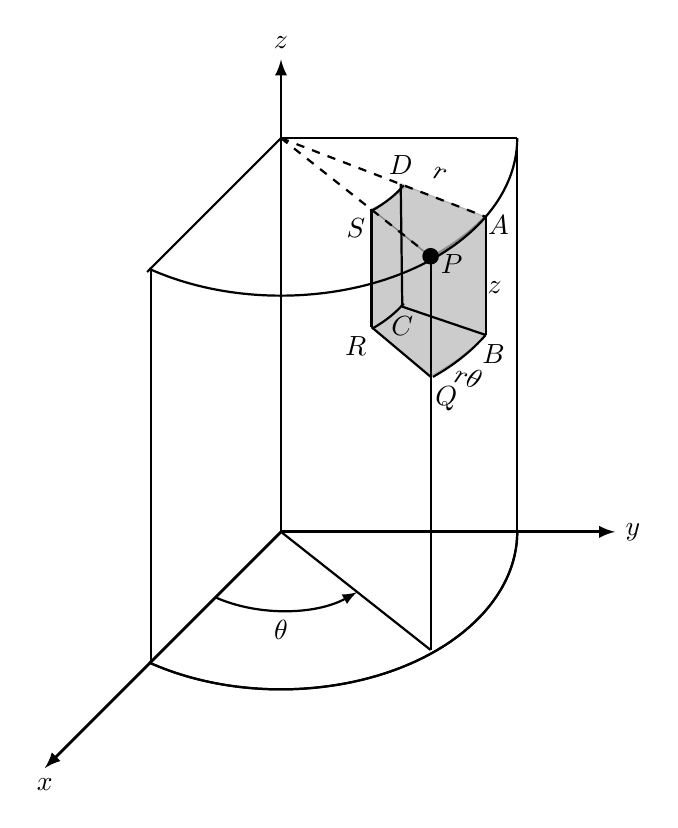
\begin{tikzpicture}[scale=1]
		\coordinate (O) at (0,0);
		\coordinate (Ox) at (-3,-3);
		\coordinate (Oy) at (4.243,0);  % sqrt{18}
		\coordinate (Oz) at (0, 6);
		
		% draw axis
		\draw[-latex, line width=1] (O)-- (Ox) node[below] {$x$};
		\draw[-latex, line width=1] (O)-- (Oy) node[right] {$y$};
		\draw[-latex, line width=1] (O)-- (Oz) node[above] {$z$};
		
		
		% draw arcs
		\draw[thick] ($(0, 0) + (236:3cm and 2cm)$(P) arc
		(236:360:3cm and 2cm);
		\draw[thick] ($(0, 0) + (236:3cm and 2cm)$(P) arc
		(236:360:3cm and 2cm);
		
		\draw[thick] ($(0, 5) + (236:3cm and 2cm)$(P) arc
		(236:360:3cm and 2cm);
		
		\draw[thick, -latex] ($(0, 0) + (236:1.5cm and 1cm)$(P) arc
		(236:310:1.5cm and 1cm);
		
		\coordinate (Phi) at (0,-1) ;
		\node[below] at (Phi) {$\theta$};
		
		
		\coordinate (A1) at (0, 5);
		\coordinate (B) at (3, 5);
		\coordinate (C) at (-1.7, 3.3);
		\draw[thick] (A1)--(B);
		\draw[thick] (A1)--(C);
		
		
		
		% radius
		\coordinate (D) at (1.9,-1.5);
		\coordinate (P) at (1.9,3.5);
		\draw[thick] (O)--(D);
		\draw[thick, dashed] (A1)--(P) node[right, yshift=-1mm] {$P$};
		\draw[thick] (D)--(P);
		\fill[black] (P) circle (3pt);
		
		
		\coordinate (A) at (2.6, 4.0);
		\draw[thick, dashed] (A1)--(A) node[right, yshift=-1mm, xshift=-1mm] {$A$};
		
		
		% arcs
		\draw[thick] ($(0, 5) + (310:1.8cm and 1.2cm)$(P) arc
		(310:330:1.8cm and 1.2cm);
		
		\draw[thick] ($(0, 3.5) + (310:1.8cm and 1.2cm)$(P) arc
		(310:330:1.8cm and 1.2cm);
		
		\draw[thick] ($(0, 3.5) + (310:3cm and 2cm)$(P) arc
		(310:330:3cm and 2cm);
		
		\coordinate (Q) at (1.9,1.97);
		\node[below,xshift=2mm] at (Q) {$Q$};
		% \fill[black] (Q) circle (3pt);
		
		
		\coordinate (B) at (2.6, 2.5);
		\node[below,xshift=1mm] at (B) {$B$};
		% \fill[black] (B) circle (3pt);
		\draw[thick] (A) --(B);
		
		\coordinate (S) at (1.15, 4.1);
		\node[below, xshift=-2mm] at (S) {$S$};
		% \fill[black] (S) circle (3pt);
		
		\coordinate (R) at (1.15, 2.6);
		\node[below, xshift=-2mm] at (R) {$R$};
		%\fill[black] (R) circle (3pt);
		
		
		\coordinate (D) at (1.52, 4.42);
		\node[above] at (D) {$D$};
		% \fill[black] (D) circle (3pt);
		
		\coordinate (C) at (1.54, 2.86);
		\node[below] at (C) {$C$};
		%\fill[black] (C) circle (3pt);
		
		\draw[thick] (S) --(R);
		\draw[thick] (D) --(C);
		\draw[thick] (R) --(Q);
		\draw[thick] (C) --(B);
		
		% verticals on the planes
		\coordinate (H) at (-1.65,-1.65);
		%\fill[black] (H) circle (3pt);
		%
		\coordinate (I) at (-1.65,3.35);
		%\fill[black] (I) circle (3pt);
		\draw[thick] (H) --(I);
		
		\coordinate (J) at (3,0);
		%\fill[black] (J) circle (3pt);
		\coordinate (K) at (3,5);
		%\fill[black] (K) circle (3pt);
		\draw[thick] (J) --(K);
		
		% filling
		\filldraw[opacity=0.2]
		(D)--(A) arc (325:306:3cm and 2.2cm)--(S)
		arc (305:325:1.8cm and 1.2cm)--cycle;
		
		\filldraw[opacity=0.2]
		(P) arc (306:325:3cm and 2.2cm)--(B)
		arc (325:306:3.0cm and 2.2cm)--cycle;
		
		\filldraw[opacity=0.2]
		(P)--(Q)--(R)--(S)--cycle;
		
		% differential labels
		\node[right, yshift=1mm,xshift=2mm, rotate=-20] at (Q) {$r \dif \theta$};
		\node[right, yshift=6mm, xshift=-1mm ] at (B) {$\dif z$};
		\node[right,xshift=3mm, yshift=2mm, rotate=-20] at (D) {$\dif r$};
		
	\end{tikzpicture}
	\refstepcounter{figure}
	
	图\thefigure: 柱坐标系\footnote{本图来自\url{https://www.latexstudio.net/index/details/index/mid/813.html}}
\end{minipage}
\begin{minipage}{0.35\textwidth}
	如图,这是一个以$x$轴为极轴的柱坐标系,$P$的坐标为$(r,\theta,z)$。
	\[\vec{OP}=\vec{r}+\vec{z}\]
	阴影部分是一个极小的体积元(这里放大绘制)。
\end{minipage}
\vspace{2ex}

在对刚体运动进行描述时,我们往往选取刚体的旋转轴作为$z$轴建立柱坐标系,然后借助柱坐标系说明其运动的相关参数。

	
\subsection[叉乘]{\itr{Cross Product}{叉乘}\labelroot{chapter3_cross_product}}
在介绍转动的有关概念前,我们还需引入叉乘这一数学工具。

由于叉乘的具体内容介绍属于线性代数与数学分析的任务,这里并不会展开讲。

叉乘可以看成这样一个运算:按顺序输入两个向量$\vec{A},\vec{B}$,输出一个特定长度且与它们都正交的向量$\vec{C}$。当然,这样的描述是不精确的,一是长度需要确定的值,二是与$\vec{A},\vec{B}$都正交的向量方向不唯一\footnote{除了$\vec{0}$,还有正反两个方向}。因此,接下来,我们要对长度和方向作出具体描述。

\begin{Itemize}
	\item 长度:$C=AB\sin\theta$,其中$\theta$是由$\vec{A}$旋转至$\vec{B}$所成的小于$\frac{\pi}{2}$的角\footnotemark 。在几何意义上,$|\vec{C}|$即是$\vec{A},\vec{B}$构成的平行四边形的面积。
	\item 方向:$\vec{C}$的方向是介绍长度时所述的$\vec{\theta}$(角度矢量的方向:\refleaftext{chapter3_direction})的方向。在几何意义上,$\vec{C}$与$\vec{A},\vec{B}$所张成平面的法向量平行。
\end{Itemize}
%\refleaf*{chapter3_direction}[-8ex]
\footnotetext{事实上,这里不规定旋转,对于长度是没有影响的。这里这么说,主要是希望在介绍长度和方向时,这个角度可以统一。回想一下,在介绍极坐标系时,我们就规定逆时针是正方向了,所以这么规定可以合理地引出正负。}

如果这么说不够直观,我们可以参考右手定则:

\begin{singlefigure}[\En{Right-Hand Rule}]{chapter3_right_hand_rule}[0.6]
	以$\vec{A}$为起始,右手手指向$\vec{B}$弯曲(取$<\frac{\pi}{2}$方向),大拇指方向为$\vec{C}$的方向\\
	我们称$\vec{A}$叉乘$\vec{B}$等于$\vec{C}$,记作$\vec{A}\times\vec{B}=\vec{C}$
\end{singlefigure}

下面不加证明地给出叉乘的有关性质和定理:
\labelroot*{chapter3_derivation}[15ex]
\labelroot*{chapter3_double_cross_product}[20ex]

\begin{Itemize}
	\item \itr{Anti-Commutative Law}{反交换律} $\vec{A}\times\vec{B}=-\vec{B}\times\vec{A}$,即交换两向量顺序,它们的夹角方向会取反。
	\item \itr{Distributive Law}{分配律} $\vec{A}\times(\vec{B}+\vec{C})=\vec{A}\times\vec{B}+\vec{A}\times\vec{C}$
	\item \itr{Derivative}{导数} $\dfrac{\dif}{\dif t}(\vec{A}\times\vec{B})=\dfrac{\dif\vec{A}}{\dif t}\times \vec{B}+\vec{A}\times\dfrac{\dif\vec{B}}{\dif t}$\labelrootmark{chapter3_derivation}\\
	\En{It is important to preserve the
		multiplicative order of A and B}\\
	鉴于反交换率,保证叉乘的顺序正确是十分重要的。
	\item \itr{Lagrange's Identity}{拉格朗日恒等式}$(\vec{A}\times\vec{B})\cdot(\vec{C}\times\vec{D})=\left|\begin{array}{cc}
		\vec{A}\cdot\vec{C}&\vec{A}\cdot\vec{D}\\
		\vec{B}\cdot\vec{C}&\vec{B}\cdot\vec{D}
	\end{array}\right|$
	\item \itr{Double Cross Product}{二重叉乘}\labelrootmark{chapter3_double_cross_product}\begin{align*}
		(\vec{A}\times\vec{B})\times\vec{C}&=(\vec{A}\cdot\vec{C})\vec{B}-(\vec{B}\cdot\vec{C})\vec{A}\\
		\vec{A}\times(\vec{B}\times\vec{C})&=(\vec{A}\cdot\vec{C})\vec{B}-(\vec{A}\cdot\vec{B})\vec{C}
	\end{align*}
	这里也可以发现,叉乘不满足结合律。
\end{Itemize}

有些同学初次看见那么多公式难免慌张。事实上,普通物理\Romannumeral{1}对于叉乘的考察非常有限,基本只要清楚定义和基本的运算律即可。
\subsection[运动学概念]{\itr{Concepts in Kinematics}{运动学概念}}
%\textit{为了保证分析的简单,除非特别说明,我们默认,选择的旋转轴方向总是与角速度方向平行}。

在定好一个柱坐标系后之后,确定刚体的角度矢量及其与时间的关系,就能确定刚体的转动。

\begin{Itemize}
	\item \itr{Angular displacement}{角位移}\footnotemark $\Delta\vec{\theta}=\vec{\theta}_f-\vec{\theta}_i$
	\item \itr{Instantaneous angular velocity}{瞬时角速度} $\vec{\omega} = \dfrac{\dif\vec{\theta}}{\dif t}$
	\item \itr{Instantaneous angular acceleration}{瞬时角加速度}  $\vec{\alpha}=\dfrac{\dif\vec{\omega}}{\dif t}$
\end{Itemize}
\footnotetext{$\vec{\theta}$的单位rad属于数学单位,它是一个无量纲量。}

\En{When rotating about
	a fixed axis, every
	particle on a rigid
	object rotates
	through the same
	angle and has the
	same angular speed
	and the same angular
	acceleration.}

平动与转动有如下关系\labelroot{chapter3_connection}:
\begin{Itemize}
	\item  \itr{arc length}{弧长} $s=r\theta$,此指圆周运动。
	\item $\vec{v}_t=\vec{\omega}\times\vec{r}$ \& $v_t=\omega r$,其中t下标指\itr{tangential}{切向},$\vec{v}_t$即同时垂直于$z$轴\footnotemark 和$\vec{r}$的速度分量。
	\item $\vec{a}_t=\vec{\alpha}\times\vec{r}$ \& $a_t=\alpha r$,$\vec{a}_t$即同时垂直于$z$轴和$\vec{r}$的加速度分量。
\end{Itemize}
\footnotetext{注意这里垂直于$z$轴的条件,我们考虑的是绕轴旋转,所以任何轴向的速度分量也不在我们研究转动的考虑之中。}

这里叉乘的先后顺序可能并不那么好记,推荐读者自己画一个圆周运动的图,用右手定则对应验证一遍如上关系,以加深理解与记忆。

\subsection[动力学概念]{\itr{Concepts in Dynamics}{动力学概念}}
在引入了叉乘(见\refleaftext{chapter3_cross_product})这一数学工具后,我们得以较为轻松地描述转动的动力学概念。

以下默认已经选定转轴\labelroot{chapter3_axis}。

\begin{Itemize}
	\item \itr{The Moment of Inertia}{转动惯量} $\displaystyle I=\sum_{i}m_ir_i^2$,其中把刚体看成由多个质点组合而成,$r_i$即是质点$m_i$的极径矢量大小。
	
	\En{The moment of inertia is a measure of the
		resistance of an object to changes in its rotational
		motion, just as mass is a measure of the tendency
		of an object to resist changes in its linear motion.}
	\item \itr{Torque}{力矩} $\vec{\tau}=\vec{r}\times\vec{F}_{/z}$,其中$\vec{r}$是力$\vec{F}$的作用点对应的极径矢量,$\vec{F}_{/z}=\vec{F}-\vec{F}_z$,$\vec{F}_z$即$\vec{F}$在$z$轴上的分矢量\labelrootmark{chapter3_lower/z}\footnotemark。
	\item \itr{Net Torque}{合外力矩} $\displaystyle\vec{\tau}_{net}=\sum_{i}\vec{\tau}_i$
	\item 类似牛顿第二定律,有:在惯性系中,$\vec{\tau}_{net}=I\vec{\alpha}$,即合外力矩等于刚体的转动惯量乘以角加速度。
\end{Itemize}
\labelroot*{chapter3_lower/z}[-22ex]
\footnotetext{事实上,力矩拥有两种定义,一种是对点定义的,为$\vec{r}\times\vec{F}$;另一种是对轴定义的,为$\vec{r}\times\vec{F}_{/z}$。鉴于我们使用了柱坐标系建立这些概念,这里选择对轴定义的力矩。}\clearpage
\begin{singlefigure}[力矩示意图]{chapter3_torque}[0.5]
	在本图中,由于$\vec{F}$没有$z$轴上的分量,所以$\vec{F}=\vec{F}_{/z}$。\\
	事实上,普物\Romannumeral{1}中基本没有出现过$\vec{F}$有$z$轴分量的情况。
\end{singlefigure}
关于以上内容的证明,见\refleaftext{prove3.1}。

其中,为了便于计算力矩,我们可以引入\itr{moment arm/force arm}{力臂}的概念,其大小即为转轴到力的作用线的距离。有了这一点,力矩的大小就可以通过力臂乘以力得到。
\begin{singlefigure}[力臂示意图]{chapter3_moment_arm}[0.45]
	$l_1$是$\vec{F}_1$的力臂,$l_2$是$\vec{F}_2$的力臂。
\end{singlefigure}

对于常见的物体,其转动惯量是应当记住的:
\begin{singlefigure}{chapter3_moment_inertia1}
\end{singlefigure}
\vspace*{-2ex}
\begin{singlefigure}[常见物体的转动惯量]{chapter3_moment_inertia2}
\end{singlefigure}
\labelroot*{chapter3_moment_inertia2}[-4ex]
对于更一般的物体,则往往通过积分的方式求取它们的转动惯量。
\section[平行轴定理/施泰纳定理]{\itr{Parallel Axis Theorem/Steiner Theorem}{平行轴定理/施泰纳定理}}
在之前对转动的动力学概念的讨论中,我们默认转轴是选定的(见\refleaftext{chapter3_axis}),这是因为,当转轴不同时,转动惯量与合力矩都会发生变化。平行轴定理是解决转轴变化过程中转动惯量变化的利器,其表述如下:
\newpage
\begin{law}[\itr{Parallel Axis Theorem/Steiner Theorem}{平行轴定理/施泰纳定理}---\refleaftext{prove3.2}]
	记刚体$M$以过质心的轴(简称质心轴)为转动轴时的转动惯量为$I_{CM}$,以任意平行于质心轴的轴为转动轴时的转动惯量为$I$,这两条轴之间的距离为$h$,则有
	\[I=I_{CM}+Mh^2\]
\end{law}

%\refleaf*{prove3.2}[-17ex]
幸于拥有平行轴公式,我们在背诵常见刚体的转动惯量时,一般只要记下其以质心轴为转动轴时的转动惯量即可。

\section[刚体中的能量]{\itr{Energy in a Rigid Body}{刚体中的能量}}
好比从牛顿三律进发到能量定律,我们将开始研究刚体中的能量。
\subsection[纯转动中的能量]{\itr{Energy in Rotation ONLY}{纯转动中的能量}}
首先,让我们思考一个只发生转动的刚体所带的能量(\refleaftext{prove3.3})。
\begin{Itemize}
	\item 动能定理 $K_R=\dfrac{1}{2}I\omega^2$
	\item 做功 $\dif W=\tau\dif\theta$
	\item 功率 $P=\tau\omega$
	\item 旋转势能 $U=\dfrac{1}{2}\kappa\theta^2$
\end{Itemize}
其中,旋转势能是指由弹性旋转体扭转回原位的趋势产生的,只依赖于其状态的能量,在数值上等于将旋
转体自原位扭转至当前位置所做的功。$\kappa$称为扭转常数,单位为$\mathrm{N}\cdot\mathrm{m}$。

当旋转体扭转了角度$\vec{\theta}$时,就会产生反力矩$\vec{\tau}=-\kappa\vec{\theta}$。
\subsection[同时发生转动与平动时的能量]{\itr{Energy in Rotation \& Translation}{同时发生转动与平动时的能量}}
现在,让我们思考一个问题:
\begin{center}
	\itshape 一个刚体在质心系中能够发生平动吗?
\end{center}

答案是否定的。如果刚体在质心系中发生平动,那么质心就会拥有平动速度,然而,在质心系中,质心又一直处于原点,这与质心拥有平动速度相矛盾,因此刚体在质心系中只能发生转动\labelroot{chapter3_rotation_CM}。

既然如此,我们便会有这样的想法:利用质心系,把同时发生平动和转动的物体转化成只发生转动的物体来研究。如此,便产生了柯尼希定理:
\begin{law}[\itr{Konig's Theorem}{柯尼希定理}---\refleaftext{prove3.4}]
	记一个系统$M$的质心速度为$v_{CM}$,在质心系中的动能为$K^{CM}$,在静止参考系中的动能为$K$,并记$K_{CM}=\dfrac{1}{2}Mv_{CM}^2$,则有
	\[K=K_{CM}+K^{CM}\]
	如果考虑对一个刚体使用柯尼希定理,则有:
	\[K=\dfrac{1}{2}Mv_{CM}{}^2+\dfrac{1}{2}I_{CM}\omega^2\]
\end{law}
%\refleaf*{prove3.4}[-34ex]

在研究一个同时发生平动和转动的物体的动能时,我们往往使用柯尼希定理,分别求解其质心的平动动能和在质心系中的转动动能。
\section[角动量]{\itr{Angular Momentum}{角动量}}
与平动时的动量类似,我们可以定义刚体的角动量。
\subsection[定义]{Definition}
\begin{Itemize}
	\item \itr{Angular Momentum}{角动量} $\displaystyle\vec{L}=\sum_i\vec{r}_i\times\vec{p}_{i/z}=I\vec{\omega}$,其中$\vec{p}_{i/z}=\vec{p}_i-\vec{p}_{iz}$,$ \vec{r}_i\times\vec{p}_{i/z}$应视作质点$m_i$的角动量。角动量的方向总是与角速度的方向一致\footnotemark。
	\item 类似动量,我们有$\dfrac{\dif \vec{L}}{\dif t}=\vec{\tau}_{net}$。
\end{Itemize}
以上内容证明见\refleaftext{prove3.5}。

\footnotetext{对于这句话需持谨慎态度。在本文所定义的概念体系中,这句话是成立的,但由于大多数对角动量的定义都是对点定义,即$\displaystyle\sum_i\vec{r}_i\times\vec{p}_i$,就出现了角动量方向与角速度方向不一致的说法。\textbf{当出现这类判断时,请优先考虑不一致的说法}。}
\subsection[角动量守恒]{\itr{Conservation of Angular Momentum}{角动量守恒}}
\begin{Itemize}
	\item \itr{Conservation of Angular Momentum}{角动量守恒}由角动量的性质,我们可以发现,当合外力矩的值为$\vec{0}$时,系统的角动量保持守恒。
	\[\vec{\tau}_{net}=0\Leftrightarrow\vec{L}=Constant\]
\end{Itemize}
利用角动量守恒,可以解释开普勒第二定律。
\begin{singlefigure}[\En{Kepler's Second Law}]{chapter3_kepler's_second_law}
	对$M_p$分析,有$\vec{\tau}_{net}=\vec{r}\times\vec{F}_g=\vec{0}$,因此角动量守恒\\[1ex]
	$\dfrac{\dif A}{\dif t}=\dfrac{1}{2}|\vec{r}\times\vec{v}|=\dfrac{L}{M_p}\Rightarrow$单位时间扫过面积相等
\end{singlefigure}
\En{When a force is directed toward or away from a
	fixed point and is function of $\vec{r}$ only, it is called a
	\itr{Central Force}{中心力}}
	
	总是可以选择合适的轴,使得中心力产生的力矩为$\vec{0}$。
	
	花样滑冰时选手收紧胳膊旋转较快,而张开双臂后旋转变
	慢,这也是角动量守恒的功劳。你可能会发现,收紧胳膊时,人的动能变大了,这是生物能的功劳。
\subsection[质心系转化]{\itr{Center of Frame Translation}{质心系转化}}
角动量在静止参考系和质心系间的转化与柯尼希定理类似。
\begin{law}[\itr{Angular Momentum Translation Using C.M. Frame}{利用质心系的角动量变换}\footnotemark---\refleaftext{prove3.6}]
	记质心角动量为$\vec{L}_{CM}=M\vec{r}_{CM}\times\vec{v}_{CM}$,刚体在质心系中的角动量为$\vec{L}^{CM}=\sum_im_i\vec{r}_i^{CM}\times\vec{v}^{CM}_i$,刚体在静止参考系中的角动量为$\vec{L}$,且保证两个参考系中选取的轴平行,则有
	\[\vec{L}=\vec{L}_{CM}+\vec{L}^{CM}\]
\end{law}
%\refleaf*{prove3.6}[-22ex]
\footnotetext{对于对点定义的角动量,也有类似的结论,证明方法也基本相同。}
\section[重心]{\itr{Center of Gravity}{重心}}
我们会注意到,在分析重力产生的合力矩时,依据定义,应该对每一个质元求分力矩,然后进行求和。这似乎是一件复杂的事情。有没有办法寻找一个点,使得刚体的合重力在此作用时,得到的力矩恰等于重力的合力矩呢?事实上,我们把这样的点称作重心。

一个重要的结论是:
\begin{center}
	{\itshape 对于均匀的重力场,刚体的重心与质心重合(\refleaftext{prove3.7})}。
\end{center}

至于不均匀的情况,就需要依据定义进行计算了。
\section[非惯性系情形]{\itr{Non-Inertial Frame Situation}{非惯性系情形}}
\subsection[非惯性力]{\itr{Inertial Force}{惯性力}}
由于转动动力学的所有定律都是基于牛顿运动定律,结合数学方法推出的,因此,对于一个拥有加速度$\vec{a}_{frame}$的平动非惯性参考系\labelroot{chapter3_translation},我们需要在分析其中的物体时添上惯性力$\vec{F}_{fictious}=-m\vec{a}_{frame}$,其中$m$为物体的质量。此时,牛顿运动定律保持成立,转动动力学中的定律也保持成立。

\subsection[科里奥利力*]{\itr{Coriolis Force}{科里奥利力}*}
你可能注意到了,之前的表述中,我们讲的是“拥有加速度$\vec{a}_{frame}$的平动非惯性参考系”(\refleaftext{chapter3_translation})。这暗示着,如果参考系还发生着转动,情况又会有所不同。

对于一个仅发生转动的参考系,有如下定理:
\begin{law}[\itr{Frame Translation with Rotation}{考虑转动的参考系变换}$^*$---\refleaftext{prove3.8}]
	如果希望牛顿运动定律在一个转动参考系$\mathcal{F}'$中依然成立,我们需要对$\mathcal{F}'$中的物体添加三个假想力,分别是$-2m\vec{\omega}\times\vec{v}',-m\vec{\alpha}\times\vec{r}',m\omega^2\vec{r}'$。
	
	其中,$\vec{\omega}$是$\mathcal{F}'$的角速度,$\vec{\alpha}$是$\mathcal{F}'$的角加速度,$\vec{v}$是物体在$\mathcal{F}'$中的速度,$\vec{r}'$是物体在$\mathcal{F}'$中的极径矢量。
	
	如果我们将条件简化,认为$\mathcal{F}'$没有角加速度,则无需考虑$-m\vec{\alpha}\times\vec{r}'$。
	
	我们称$-2m\vec{\omega}\times\vec{v}'$为\itr{Coriolis Force}{科里奥利力},$m\omega^2\vec{r}'$为\itr{Centrifugal Force}{离心力}。
\end{law}
\begin{singlefigure}[地球的科里奥利力]{chapter3_earth}[0.42]
如果考虑地球的科里奥利力,我们会发现,在北半球上,\\科里奥利
力永远指向物体运动方向的右侧,而在南半球正好相反。
\end{singlefigure}
台风的旋转方向在北半球是逆时针,在南半球是顺时针,这也是科里奥利力的影响。

{\bfseries 科里奥利力是一种假想力}\footnote{我们有时会看见类似“科里奥利力是由于地球自转而施加给地球上的物体的力”的说法,这么讲可能是因为我们往往以地球为参考系分析问题,此时要想保证牛顿第二定律成立,就要认为物体受到科里奥利力。不过,一般而言,科里奥利力较小,在日常生活的分析中大多可忽略不计。}。
\section[回顾与总结]{Review and Summary}
在我们的推导中,我们发现,转动力学的结论与平动力学有着惊人的相似性。关注这份相似性既能体会物理的美感,又能加深对结论的记忆。
\[\ \ \begin{aligned}
	&\mathrm{Angular~speed~}\vec{\omega}=\dif\vec{\theta}/\dif t&& \mathrm{Linear~speed~}\vec{v}=\dif \vec{x}/\dif t  \\
	&\mathrm{Angular~acceleration~}\vec{\alpha}=\dif\vec{\omega}/\dif t&& \mathrm{Linear~acceleration~}\vec{a}=\dif \vec{v}/\dif t  \\
	&\mathrm{Resultant~torque~}\sum\vec{\tau}=I\vec{\alpha} && \mathrm{Resultant~force~}\sum \vec{F}=m\vec{a}  \\
	&\begin{array}{l}{{\mathrm{If}}}\\{\vec{\alpha}=\mathrm{constant}}\left\{\begin{array}{l}{{\vec{\omega}_{f}=\vec{\omega}_{i}+\vec{\alpha} t}}\\{{\vec{\theta}_{f}-\vec{\theta}_{i}=\vec{\omega}_{i}t+\frac{1}{2}\vec{\alpha} t^{2}}}\\{{\omega_{f}{}^{2}=\omega_{i}{}^{2}+2\alpha(\theta_{f}-\theta_{i})}}\end{array}\right.\end{array}
	&&
	\begin{array}{l}{{\mathrm{If}}}\\{\vec{a}=\mathrm{constant}}\left\{\begin{array}{l}{{\vec{v}_{f}=\vec{v}_{i}+\vec{a}t}}\\{{\vec{x}_{f}-\vec{x}_{i}=\vec{v}_{i}t+\frac{1}{2}\vec{a}t^{2}}}\\{{v_{f}{}^{2}=v_{i}{}^{2}+2a(x_{f}-x_{i})}}\end{array}\right.\end{array}  \\
	&\mathrm{Work}\ W=\int_{\theta_{i}}^{\theta_{f}}\tau d\theta && \mathrm{Work}\ W=\int_{x_{i}}^{x_{f}}F_{x}dx  \\
	&\mathrm{Rotational~kinetic~energy~}K_{\mathrm{R}}=\frac{1}{2}I\omega^{2}&& \mathrm{Kinetic~energy~}K=\frac{1}{2}mv^{2}  \\
	&\mathrm{Power}\ P=\vec{\tau}\cdot\vec{\omega}&& \mathrm{Power}\ P=\vec{F}\cdot\vec{v}  \\
	&\mathrm{Angular~momentum~}\vec{L}=I\vec{\omega} && \mathrm{Linear~momentum~}\vec{p}=m\vec{v}  \\
	&\mathrm{Resultant~torque~}\sum\vec{\tau}=\dif \vec{L}/\dif t&& \mathrm{Resultant~force~}\sum \vec{F}=\dif \vec{p}/\dif t 
\end{aligned}\]




  







	\newpage
\section{课后习题:转动动力学}
\begin{example}[{\small Determine the Moment of Inertia of an Irregularly Shaped Object}---\refleaftext{solution3.1}]
	This problem describes one experimental method of
	determining the moment of inertia of an irregularly
	shaped object such as the \itr{payload}{有效负载} for a satellite. 
	\begin{center}
		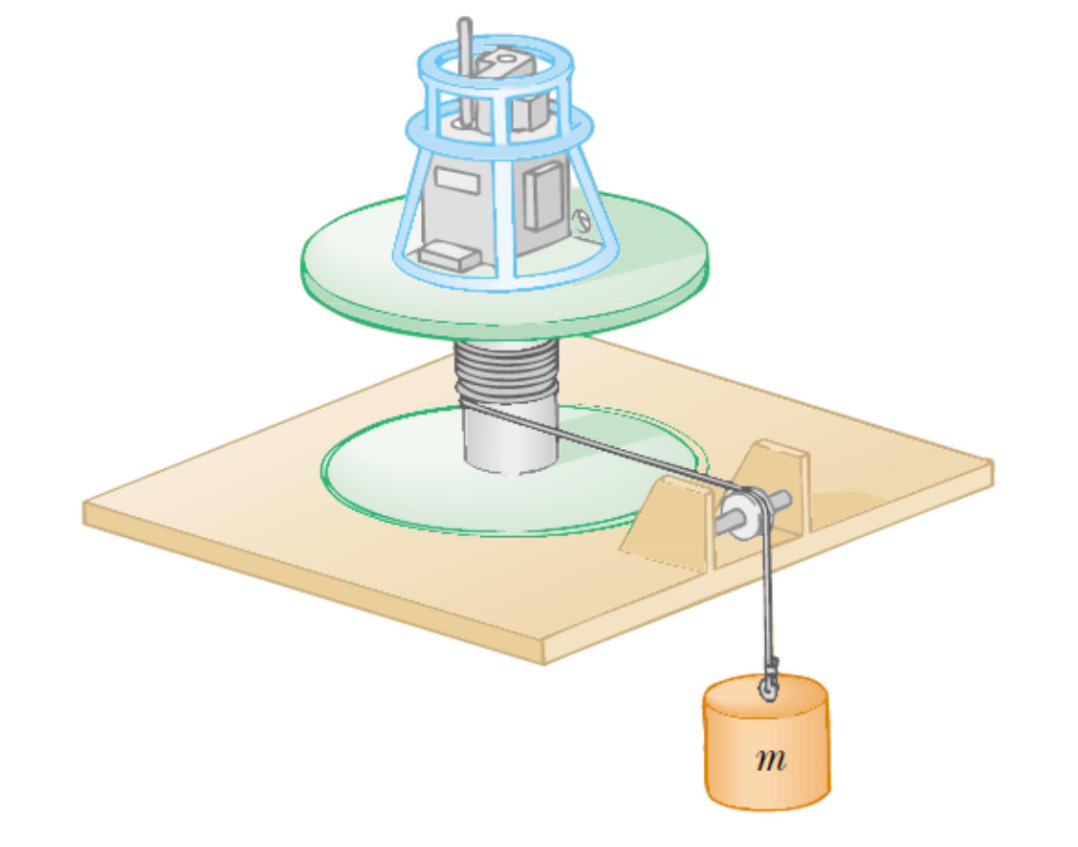
\includegraphics[width=0.6\textwidth]{chapter3_example_1}
	\end{center}
	
	The figure shows a mass $m$ \itr{suspended}{悬挂} by a \itr{cord}{绳子} \itr{wound}{被缠绕}
	around a spool of radius $r$, forming part of a \itr{turntable}{转台}
	supporting the object. When the mass is released from
	rest, it \itr{descends}{下降} through a distance $h$, acquiring a speed
	$\vec{v}$. Show that the moment of inertia $I$ of the equipment
	(including the turntable) is\quad$mr^2(\dfrac{2gh}{v^2}-1)$. 
\end{example}
%\refleaf*{solution3.1}[-75ex]
\begin{example}[Rolling Items---\refleaftext{solution3.2}]
	Three objects of \itr{uniform density}{均匀的密度} --- a \itr{solid sphere}{实心球}, a \itr{solid
	cylinder}{实心圆柱}, and a \itr{hollow cylinder}{空心圆柱} --- are placed at the top of
	an \itr{incline}{斜坡}. 
	\begin{center}
		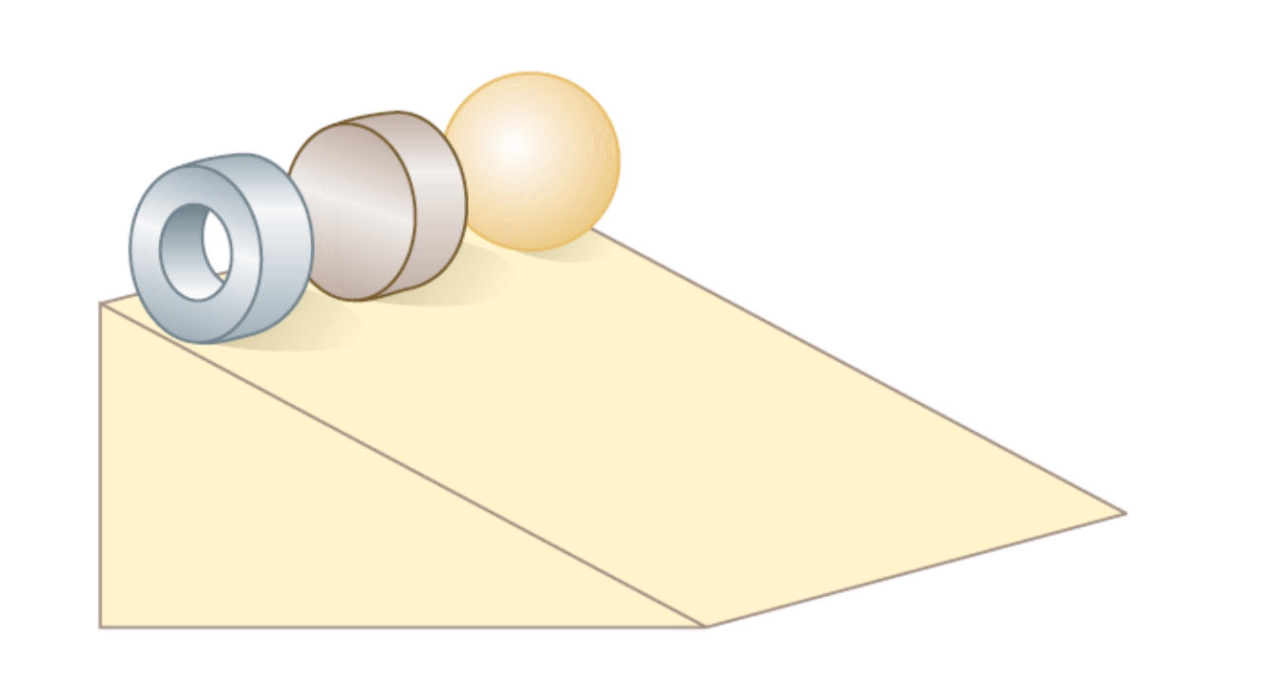
\includegraphics[width=0.6\textwidth]{chapter3_example_2}
	\end{center}
	If they all are released from rest
	at the same \itr{elevation}{高度} and roll without \itr{slipping}{滑动}, which object reaches the bottom first?
\end{example}
%\refleaf*{solution3.2}[-20ex]
\begin{example}[Calculation of the Moment of Inertia---\refleaftext{solution3.3}]
	A rod's \itr{linear density}{线密度} is given by $\lambda=kx$, where $x$ represents the distance from the point to the rod's center. 
	\begin{singlefigure}{chapter3_rod}[0.5]
	\end{singlefigure}
	Given the length of the rod $l$, try to calculate the moment of inertia of the rod, given the rotation axis at:
	
	(1) Center $O$ as the $y$ axis shows.
	
	(2) One end as the $y'$ axis shows.
\end{example}
\begin{example}[Massive \itr{Pulley}{滑轮}---\refleaftext{solution3.4}]
	Consider two \itr{cylinders}{圆柱} having masses $m_1$
	and $m_2$, where $m_1 < m_2$, connected by a
	string passing over a pulley. The pulley
	has a radius $R$ and moment of inertia $I$
	about its axis of rotation.
	\begin{singlefigure}{chapter3_massive_pulley}[0.3]
		The string does
		not \itr{slip}{滑动} on the pulley, and the system
		is released from rest. 
	\end{singlefigure}
	 Find the linear
	speeds of the cylinders after
	cylinder 2 \itr{descends}{下降} through a
	distance $h$, and the angular
	speed $\omega$ of the pulley at this time.
\end{example}
\begin{example}[Object rotating on a string
	of changing length---\refleaftext{solution3.5}]
	Initially, the mass \itr{revolves}{转动} with a speed $v_1$ = 2.4 m/s in
	a circle of radius $R_1$ = 0.80 m.
	The string is then pulled slowly through the hole so
	that the radius is reduced to $R_2$ = 0.48 m. What is the
	speed, $v_2$, of the mass now?
	\begin{singlefigure}{chapter3_string}[0.7]
	\end{singlefigure}
\end{example}
\begin{example}[Rotation of a sliding rigid rod---\refleaftext{solution3.6}]
	Consider a rod with mass m and length L standing straight on the friction-less ground. When we
	release the rod, it will fall from the unstable \itr{equilibrium position}{平衡位置}.
	\begin{center}
		\begin{minipage}{0.45\textwidth}
			\centering
			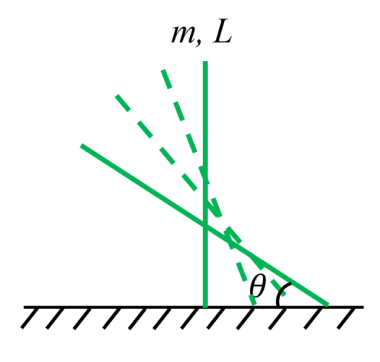
\includegraphics[width=\linewidth]{chapter3_rotating_rod_1}\\
			Figure 1
		\end{minipage}
		\quad
		\begin{minipage}{0.45\textwidth}
			\centering
			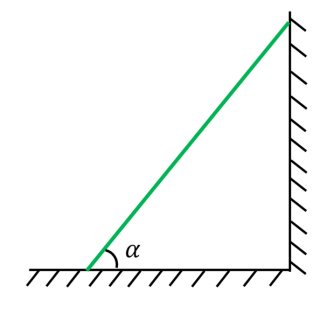
\includegraphics[width=\linewidth]{chapter3_rotating_rod_2}\\
			Figure 2
		\end{minipage}
	\end{center}
	(a) Calculate the angular velocity of the rod, when it has an angle of $\theta$ with respect to the ground
	as illustrated in Figure 1.\\
	(b) What is the final angular velocity $\omega_1$ of the rod before it hits the ground?\\
	(c) If the same rod is leaning to a frictionless wall with an initial angle of α to the frictionless
	ground (see Figure 2), what is the final angular velocity $\omega_2$ of the rod before it hits the ground?\\
	{\em Note that there is a possibility that the right end of the rod leaves from the wall before the rod hits the ground.}
\end{example}
	\begin{comment}
    \documentclass{Physics_H_Notes}
    \usepackage{upgreek}
    \begin{document}
    \end{comment}
        \chapter[流体力学]{\itr{Fluid Mechanics}{流体力学}}
        本章节存在一定的特殊性:在2022年及之前,流体力学是普物\Romannumeral{1}的内容,而在2023级,这一块内容被路欣老师为代表的教学组删去了。

        当看到流体力学的时候,你想到的是什么?或许是初中的水的压强,又或者是湍流等复杂情景。其实都无所谓,毕竟它们都是流体的研究。当今世界对于流体力学的探究也是一个重要的力学方向,小到潜水,大到飞机飞船,都需要关注流体对于物体的影响。
        但是,我们这门课程的流体力学相当简单和浅层,按照笔者当时授课较为简单的pzq老师的内容,我用一句话定义这一块内容:两个公式走天下!这是由于我们使用了大量的理想情景,抛除复杂情景所致。
        \section[流体的定义与性质]{\itr{Definition \& Properties of Fluids}{流体的定义与性质}}
        生活中的物体可分为固体、液体和气体三大类,其中,我们一般将液体和气体统称为流体。它们一般受到的力是不一样的:
        \begin{Itemize}
            \item \itr{solid}{固体}:\itr{compression force}{压缩力}(指物体能够从两侧被挤压), \itr{tensile force}{拉力}(指物体能够受力被拉伸), 
                \itr{shearing force}{剪切力}(指物体能够受到不在同一直线上的两个相反方向的力而保持形状不变)
            \item \itr{liquid}{液体}:compression force, tensile force, no shearing force
            \item \itr{gas}{气体}:compression force, no tensile force, no shearing force
        \end{Itemize}
        
        在静止的液体中,我们已经了解到物体一定会受到水的压力,进而定义压强。
        \begin{law}[静止流体中的压强]
            利用微元法分析,我们可以知道物体受到的静止流体的压强为:
            \begin{center}
                $\dfrac{dp}{dy}=-\rho g$,积分可得$p=p_0+\rho gh$
            \end{center}

            其中$p_0$是液体表面的压力,$h$为深度,$y$为该点相对于参考平面的高度。
        \end{law}
        
        对于静止流体,我们也有两个重要的而且很直观的性质:
        \begin{law}[\itr{Pascal's Principle}{帕斯卡原理}]
            施加在封闭流体上的力被不减弱地传递到流体的每一部分和容器的壁上。假设流体中受力面积为$S$的某点处原有压强为$p_0$,在其上方平面施加垂直向下的力F,则该点处当前的压力为:
            \begin{center}
                $F^{'}=p_0 S +F$
            \end{center}
        \end{law}

        这是很容易理解的,我们以按压海绵为例,力的作用会逐渐传导到物体的每个位置。当然,帕斯卡原理强调了在流体中这个力是不会减弱的,
        而海绵是固体,力是会减弱的。
        \begin{law}[\itr{Archimedes's Principle}{阿基米德原理}]
            一个部分或者完全浸入液体中的物体受到的浮力等同于它所排出的液体的重力。
        \end{law}

        最简单的例子,就是我们初中学过的物体受到水的浮力的公式:
        \begin{center}
            $F=\rho gV$
        \end{center}

        我们可以很容易地知道这个公式的本质就是阿基米德原理。

        在液体中存在表面张力,表面张力是一种由于液体分子间的相互吸引与拉扯而产生的力的作用,其大小与物体间的接触长度有关。定义表面张力系数为:
        \begin{center}
            $\gamma =\dfrac{F}{l}$
        \end{center}

        其中$F$为该处受到的表面张力大小,$l$表示接触面的长度。这里的表面张力定义与普通化学(H)中的定义相同。当表面张力产生时,由于物体具有一定厚度,
        一般情况下会产生两个液体膜的拉力作用,因此计算时通常需要将长度以两倍长度,即$2l$计算。

        由于物体与液体间的表面张力系数不同,会产生浸润与非浸润的区别。这个概念与普化课程一致,且一般不作考察,因此我们暂不讨论。
        \section[流体动力学]{\itr{Fluid Dynamics}{流体动力学}}
        或许你一直有疑问:我感觉我也没学啥呀,怎么就动力学了?确实,我们到目前的流体力学都是初中水平。而接下来,就是流体力学两个方程走天下的经典例子。
        
        我们定义流体的通量为:$Q=\dfrac{\delta m}{\delta t}=\rho Av$,表示单位时间内流过截面积为$A$的流体的质量,其中$\rho$表示流体密度,$A$表示流体通过的截面面积,$v$表示通过这个截面时的流体流速。
        首先考虑一个水管,里面充满了水,水管不可压缩变形,水也不可压缩变形。那么很明显,水管的一端进入多少水,另一端就会有多少水流出。
        \begin{law}[管流原理(连续性原理)]
            流体流入某个管的通量等于流出该管的通量,即:$\rho_1 A_1 v_1=\rho_2 A_2 v_2$
        \end{law}

        在这个方程中,我们看到了同一个流体的管流特点。当然,这个方程忽略了压强和位置的变化。因此,我们针对理想流体,即不可被压缩、遵循管流原理、没有湍流现象或其他扰动的流体,提出了伯努利方程:
        \begin{law}[\itr{Bernoulli’s Equation}{伯努利方程}]
            \centering
            $\dfrac{1}{2}\rho v^2 +p+\rho gy=constant$
        \end{law}

        只需要在使用中注意的一点是,这里的$y$表示的是位置相对于参考平面的高度,而非相对于液面的深度。在满足上述条件的情况下,只要是同一个连通的流体,在其内部每一点处,上述等式左边的结果均相等。

        当然,看到这里,我们已经了解了两个重要的方程。结合中学的压强的定义,我们已经可以用两个方程大步走入流体力学的世界了。最后,这些已经足够我们普物的内容了,更为复杂的情况,交给流体力学的专家们解决吧
        %\end{document}
	\section{课后习题:流体力学}
	\begin{example}[流体静力学---\refleaftext{solution4.1}]
		A fluid is rotating at constant angular velocity $\omega$ about the central vertical axis of a cylindrical container.As shown in Figure 4-1:
		\begin{singlefigure}[流体静力学]{chapter4_流体静力学}[0.45]
		\end{singlefigure}
		
		(a)Show that the \itr{variation}{变化} of pressure in the \itr{radial direction}{径向} is given by $\dfrac{\dif p}{\dif r}=\rho \omega^2 r$.
		
		(b)Take $p=p_c$ at the axis of rotation ($r=0$) and show that the pressure $p$ at any point $r$ is
		\begin{center}
			$p=p_c+\dfrac{1}{2}\rho\omega^2 r^2$
		\end{center}

		(c)Show that the liquid surface is of \itr{paraboloidal}{抛物面的} form(Figure 4-1); that is, a vertical cross section of the surface is the curve $y=\dfrac{\omega^2 r^2}{2g}$
	\end{example}
	%\refleaf*{solution4.1}[-107ex]
	\begin{example}[流体动力学---\refleaftext{solution4.2}]
		As shown in Figure 4-2, it is an \itr{air suction device}{空吸装置}. Given that the depth of the centerline of the \itr{catheter}{导管} below the liquid level in container $A$ is $h$, 
		the height difference between the liquid level in container $B$ and the centerline of the horizontal catheter is $h_b$, \itr{the cross-sectional area}{横截面积} at the \itr{nozzle}{喷嘴} $d$ is $S_d$, 
		and the cross-sectional area at the \itr{contraction section}{收缩段} $c$ is $S_c$. What are the conditions for the \itr{ratio}{比率} of $S_d$ to $S_c$ to occur for \itr{suction}{抽吸}?
		\begin{singlefigure}[流体动力学]{chapter4_流体动力学}[0.65]
		\end{singlefigure}
	\end{example}
	%\refleaf*{solution4.2}[-83ex]
	%\input{../chapters/chapter5/chapter5_main}
	%\input{../chapters/chapter5/chapter5_exercise}
	\chapter[狭义相对论]{\itr{Special relativity}{狭义相对论}}
进入狭义相对论,我们就开始从熟悉的三维世界来到了陌生的四维世界。作为三维世界的生物大家都一样,谁都没有进化出适用于四维空间的大脑。也许我们并不能建立对于四维世界的直观认知——\begin{center}
	\itshape 我们能做的,仅仅是通过一些抽象的数学工具来尝试刻画这个神秘而又复杂的四维空间。
\end{center}
\section[相对论运动学]{\itr{Time and Space in Special relativity}{相对论运动学}}
在开始我们的讨论前,有必要先强调一下如下概念:
\begin{description}
	\item[同一事件] 我们要注意的是,在狭义相对论中,只有\textbf{同时同地发生}的事件才叫做同一事件,同一事件是无论在哪个参考系中都要承认的\footnote{\eg 若$S$系中的李同学在自己的钟读数为5:00时,与$S'$系中的王同学在同一位置相遇,并看见王同学的钟读数为4:00,那么,王同学也必须承认,当自己的钟读数为4:00时,他与李同学相遇且看到李同学的钟读数为5:00。}。
	\item[观察与“看”] 在狭义相对论中的题目中,我们遇到的大部分情形是观察。比如说,“在地面系看来火车系上的追击过程花了多久时间”,这种“看”应该理解为观察,也就是通过实验、测量等方式,以一种上帝视角\mgnote{可以有无数个在同一个系里的观察者}[-6ex]得出的结果\mgnote{也就是用洛伦兹变换(\refleaftext{chapter_6_Lorentz_Transformation})得到的结果};我们也许还会遇到一种“看”,这种看应该理解为一个单独的观察者所观察到的情况,如“高速运动的物体的视觉效应”。我们之后的练习也会涉及到这一点。
\end{description}
\subsection[基本假设]{\itr{Basic assumptions}{基本假设}}

\begin{Itemize}
    \item \itr{Principle of the Constancy of Lightspeed}{光速不变性原理}\ 光速与光源和接收器的运动无关。
    \item \itr{The Principle of Relativity}{相对性假设}\ 对于任何两个匀速运动的观察者来说,基本物理定律完全相同。(相对性假设)
\end{Itemize}
\subsection[洛伦兹变换]{\itr{Lorentz Transformation}{洛伦兹变换}}
洛伦兹变换是狭义相对论的核心。在理解种种狭义相对论现象之前,我们不妨先引入洛伦兹变换。
\labelroot*{chapter_6_Lorentz_Transformation}[45ex]
\begin{law}[\itr{Lorentz Transformation}{洛伦兹变换}]
	\begin{singlefigure}[洛伦兹变换]{chapter_6_Lorentz_Transformation}[0.4]
	\end{singlefigure}
	设$S'$系相对$S$系有$x$方向的速度$v$,并分别用$t,t'$表示$S$系,$S'$系中的时间,用$x,y,z$与$x',y',z'$表示$S$系,$S'$系中的坐标,则有
	\[
		\left\{
			\begin{array}{l}
				t'=\gamma(t-\beta x/c)\\
				x^{\prime}=\gamma(x-vt)\\
				y^{\prime}=y\\
				z^{\prime}=z
			\end{array}
		\right.
	\]
	其中 $\gamma = \dfrac{1}{\sqrt{1-v^2/c^2}} \quad,\quad\beta=\dfrac{v}{c}$。
\end{law}

注意到这里我们仅仅介绍了正逆变换中的一个。实际上,由基本假设2(相对性假设)可知,无论在哪个参考系下,洛伦兹变换都应该具有
相同的形式。所以,我们自然而然的引入一种符号法则,即给$v$带上正负号,并约定:
\begin{center}
	\itshape 在等号左边的系看来,等号右边的系沿着等号左边的系的正方向运动时,$v$取正号;负方向运动时,$v$取负号。
\end{center}

比如说,在定理说明时,$S$系沿着$S'$系的负方向运动,所以$v$前与$\beta$前取负号。
\subsection[动尺收缩]{\itr{Lorentz Contradiction}{动尺收缩}}
\begin{singlefigure}{chapter_6_2}[0.45]
\end{singlefigure}
考虑一根在参考系S静止的杆,它顺着x轴放置。因为杆在S系中静止,其端点的位置坐标$x_1$和$x_2$与时间无关。因此,
\[L_0=x_2-x_1\]
被称为杆的\textbf{原长}或\textbf{静止长度}。\\
下记$S'$系中测量杆长的结果为$L$,由洛伦兹变换有
\[x_{1}=\gamma\left(x_{1}^{\prime}+vt_{1}^{\prime}\right), \]
\[x_{2}=\gamma\left(x_{2}^{\prime}+vt_{2}^{\prime}\right), \]
于是有
\[x_{2}-x_{1}=L_{0}=\gamma\left(x_{2}^{\prime}-x_{1}^{\prime}\right)+\gamma v\left(t_{2}^{\prime}-t_{1}^{\prime}\right) \]
由于我们是在$S^{\prime}$系下做的测量,故令$t_{2}^{\prime}=t_{1}^{\prime}$,从而得到
\[L_0=\gamma L\]
由上述讨论,我们不难发现,之所以尺子会变短,是因为我们的测量出了问题:
\begin{center}
	\itshape 我们的测量仅仅保证了在$S$系下是同时的。\\然而,在$S^{\prime}$系看来,这两种操作并不是同时的。
\end{center}

事实上,在$S^{\prime}$看来,$S$系进行的测量是先测的头后测的尾,其仅仅测量了尺子的一部分,故必然会得到尺缩的结论。
\subsection[动钟变慢]{\itr{Time dilation}{动钟变慢}}
在时钟静止的参考系中,时间间隔的测量结果记为
\[\tau=t_2-t_1\] 
它称为\textbf{原时}或\textbf{本征时间}。然后我们用洛伦兹变换得到
\[t_{2}'=\gamma\left(t_{2}-\frac{\beta x_{2}}{c}\right),\]
\[t_{1}'=\gamma\left(t_{1}-\frac{\beta x_{1}}{c}\right),\]
注意到我们是在$S^{\prime}$系下测量$S$系下同一处的钟的时间,故有$x_2-x_1=0$,所以可得
\[t_{2}'-t_{1}'=\gamma \tau\]
实际上,我们之所以会得到如此结果,是因为光速不变这条基本假设。由于在$S$中静止的钟在$S^{\prime}$下却是运动的,这两个事件在$S$看来不是同地发生的。由于光速不变,这两个信息以光速传播到$S$中的观察者时,必然会产生一个时间差,故看起来就像时间膨胀了一样。
\subsection[速度变换]{\itr{Speed Transformation}{速度变换}}
\begin{law}[\itr{Speed Transformation}{速度变换}]
    \[u_{x}=\frac{u_{x}^{\prime}+v}{1+\frac{v}{c^{2}}u_{x}^{\prime}},\]
    \[u_{y}=\frac{\sqrt{1-\beta^{2}}u_{y}^{\prime}}{1+\frac{v}{c^{2}}u_{x}^{\prime}},\]
    \[u_{z}=\frac{\sqrt{1-\beta^{2}}u_{z}^{\prime}}{1+\frac{v}{c^{2}}u_{x}^{\prime}}\]
\end{law}
同样的我们约定一种符号法则,v正负号的选取和洛伦兹变换一样,即等号左边的参考系看来右边的参考系相对左边参考系向正方向运动就取正号反之取负号;其他的速度如$u_{x}$,$u_{y}$,$u_{z}$其在相应的参考系下朝正半轴运动就取正号反之取负号,所得到的$u_{x}^{\prime}$,$u_{y}^{\prime}$,$u_{z}^{\prime}$也满足上述符号法则。

	\input{../chapters/chapter6/chapter6_exercise}
 	\input{../chapters/chapter7/chapter7_main}
  	\input{../chapters/chapter7/chapter7_exercise}
	\apart{证明部分}
	\chapter[测量]{\itr{Measurement}{测量}}

{\LARGE \centering \color{red}\itshape
	BLANK\\
	期待你的建设
	
}
	\chapter{}
	\chapter[转动动力学]{\itr{Rotation Dynamics}{转动动力学}}
\begin{prove}[Concepts in Dynamics\qquad$\vec{\tau}_{net}=I\vec{\alpha}$]
	要搞清楚的一点是,我们依旧基于牛顿力学来思考有关转动的问题。
	
	我们先承认一件事实:刚体的内部存在着非常复杂的相互作用力,这些作用力合理地分配,最终使得整个刚体可以做转动。于是,任意取一个质元$\dif m$分析,都有\[\dif \vec{F}_t=\dif m\vec{a}_t\]
	
	依据平动和转动的联系(见\refleaftext{chapter3_connection}),我们有
	\[\vec{a}_t\dif m=(\vec{\alpha}\times\vec{r})\dif m\]
	于是在等式两侧同左叉乘以$\vec{r}$,即有
	\[\vec{r}\times\dif\vec{F}_t= (\vec{r}\times\vec{\alpha}\times\vec{r})\dif m\]
	由双重叉乘的运算律(见\refleaftext{chapter3_double_cross_product}),知
	\[\vec{r}\times\vec{\alpha}\times\vec{r}=(\vec{r}\cdot\vec{r})\vec{\alpha}-(\vec{\alpha}\cdot\vec{r})\vec{r}=r^2\vec{\alpha}\]
	注意到
	\[\vec{r}\times\dif\vec{F}_t=\vec{r}\times\dif\vec{F}_{/z}\]
	即得
	\[\vec{r}\times\dif\vec{F}_{/z}=r^2\vec{\alpha}\dif m\Leftrightarrow\dif\vec{\tau}=r^2\vec{\alpha}\dif m\]
	等式两侧取积分,即有
	\[\vec{\tau}_{net}=I\vec{\alpha}\]
\end{prove}
%\refleaf*{chapter3_connection}[-64ex]
%\refleaf*{chapter3_double_cross_product}[-40ex]
%\newpage
\newpage
\begin{prove}[\itr{Parallel Axis Theorem}{平行轴定理}\qquad$I=I_{CM}+Mh^2$]
	不妨设$\vec{h}$的方向为从质心轴到任意轴,并取任意一质点$m_i$,其在选择质心轴时,位矢为$\vec{r}_{CMi}$,选择任意轴时,位矢为$\vec{r}_i$,则有\[\vec{r}_i=\vec{r}_{CMi}-\vec{h}\]
	于是有
	\begin{align*}
		I&=\sum_{i}m_i(\vec{r}_{CMi}-\vec{h})^2\\
		&=\sum_{i}m_i(r_{CMi}{}^2+h^2-2\vec{r}_{CMi}\cdot\vec{h})\\
		&=\sum_{i}m_ir_{CMi}{}^2+\sum_{i}m_ih^2-2\vec{h}\cdot\sum_{i}m_i\vec{r}_{CMi}\\
		&=I_{CM}+Mh^2+0\qquad(\text{由质心的性质知最后一项为0})\\
		&=I_{CM}+Mh^2
	\end{align*}
\end{prove}
\begin{prove}[Energy in Rotation ONLY]
	在只发生转动的物体中,有\[v=v_t=\omega r\]于是有
	\begin{align*}
		K_R&=\sum_i\dfrac{1}{2}m_iv_i{}^2&U&=\int_0^{\theta}\kappa\alpha\dif\alpha\\
		&=\sum_i(\dfrac{1}{2}m_i r_i{}^2)\omega^2&&=\dfrac{1}{2}\kappa\alpha^2\left|_0^{\theta}\right.\\
		&=I\omega^2&&=\dfrac{1}{2}\kappa\theta^2\\
		P&=\vec{F}\cdot \vec{v}&\dif W&=\vec{F}\cdot\dif \vec{x}\\
		&=F_tv&&=F_t\dif x\\
		&=F_tr_\omega&&=F_tr\dif\theta\\
		&=\tau\omega&&=\tau\dif\theta
	\end{align*}
\end{prove}
%\newpage
\begin{prove}[\itr{Konig's Theorem}{柯尼希定理}\qquad$K=K_{CM}+K^{CM}$]
	我们取质点$m_i$,记它在静止参考系中的速度为$\vec{v}_i$,在质心系中的速度为$\vec{v}^{CM}_i$,并记刚体的质心速度为$\vec{v}_{CM}$,则有
	\[\vec{v}_i=\vec{v}_i^{CM}+\vec{v}_{CM}\]
	于是有
	\begin{align*}
		K&=\sum_i\dfrac{1}{2}m_i(\vec{v}_i^{CM}+\vec{v}_{CM})^2\\
		&=\sum_i\dfrac{1}{2}m_i{v_i^{CM}}^2+\sum_i\dfrac{1}{2}m_i{v_{CM}}^2+(\sum_im_i\vec{v}_i^{CM})\cdot\vec{v}_{CM}\\
		&=K^{CM}+K_{CM}\qquad(\text{由质心定义知前式最后一项为0})
	\end{align*}
	由刚体在质心系中只存在转动(见\refleaftext{chapter3_rotation_CM}),有
	\[K^{CM}=\dfrac{1}{2}I_{CM}\omega^2\]
	于是
	\[K=\dfrac{1}{2}M{v_{CM}}^2+\dfrac{1}{2}I_{CM}\omega^2\]
\end{prove}
%\refleaf*{chapter3_rotation_CM}[-22ex]
%\newpage
\begin{prove}[Angular Momentum\qquad$\displaystyle\vec{L}=\sum_i\vec{r}_i\times\vec{p}_{i/z}=I\vec{\omega}\quad\&\quad\dfrac{\dif \vec{L}}{\dif t}=\vec{\tau}$]
	\qquad
	$
	\begin{array}{r@{\ }l}
		\vec{L}&=\displaystyle\sum_i\vec{r}_i\times\vec{p}_{i/z}\\
		&=\displaystyle\sum_im_i\vec{r}_i\times(\vec{v}_{ir}+\vec{v}_{it})\\
		&=\displaystyle\sum_im_i(\vec{r}_i\times\vec{v}_{ir}+\vec{r}_i\times\vec{v}_{it})\\
		&=\displaystyle\sum_im_i(\vec{0}+\vec{r}_i\times(\vec{\omega}\times\vec{r}_i))\\
		&=\displaystyle\sum_im_i((\vec{r}_i\cdot\vec{r}_i)\vec{\omega}+(\vec{r_i}\cdot\vec{\omega})\vec{r}_i)\\
		&=\displaystyle\sum_im_ir_i{}^2\vec{\omega}\\
		&=I\vec{\omega}
	\end{array}$有关双重叉乘见\refleaftext{chapter3_double_cross_product}
	\\[2ex]
	\hspace*{0.9em}
	$
	\begin{array}{r@{\ }l}
		\dfrac{\dif\vec{L}}{\dif t}&=\dfrac{\dif\displaystyle\sum_i(\vec{r}_i\times\vec{p}_{i/z})}{\dif t}\\[1.4ex]
		&=\displaystyle\sum_i\dfrac{\dif(\vec{r}_i\times\vec{p}_{i/z})}{\dif t}\\
		&=\displaystyle\sum_i(\dfrac{\dif\vec{r}_i}{\dif t}\times\vec{p}_{i/z}+\vec{r}_i\times\dfrac{\dif\vec{p}_{i/z}}{\dif t})\\
		&=\displaystyle\sum_i(\vec{v}_{i/z}\times\vec{p}_{i/z}+\vec{r}_i\times\vec{F}_{i/z})\\
		&=\displaystyle\sum_i\vec{r}_i\times\vec{F}_{i/z}\\
		&=\vec{\tau}_{net}
	\end{array}$
	有关微分见\refleaftext{chapter3_derivation}
\end{prove}
%\refleaf*{chapter3_double_cross_product}[-62ex]
%\refleaf*{chapter3_derivation}[-23ex]
\begin{prove}[$\vec{L}=\vec{L}_{CM}+\vec{L}^{CM}$]
	我们取质点$m_i$,记它在静止参考系中的速度为$\vec{v}_i$,极径矢量为$\vec{r}_i$在质心系中的速度为$\vec{v}^{CM}_i$,极径矢量为$\vec{r}_i^{CM}$,并记刚体在静止参考系中的质心速度为$\vec{v}_{CM}$,极径矢量为$\vec{r}_{CM}$则有
	\[\vec{v}_i=\vec{v}_i^{CM}+\vec{v}_{CM}\]
	\[\vec{r}_i=\vec{r}_i^{CM}+\vec{r}_{CM}\]
	于是有
	\begin{align*}
		\vec{L}&=\sum_im_i\vec{r}_i\times v_i\\
		&=\sum_im_i(\vec{r}_i^{CM}+\vec{r}_{CM})(\vec{v}_i^{CM}+\vec{v}_{CM})\\
		&=\sum_im_i\vec{r}_i^{CM}\times\vec{v}_i^{CM}+\sum_im_i\vec{r}_{CM}\times\vec{v}_{CM}\\
		&+(\sum_im_ir_i^{CM})\times\vec{v}_{CM}+\vec{r}_{CM}\times(\sum_im_i\vec{v}_i^{CM})\\
		&=\vec{L}^{CM}+\vec{L}_{CM}+\vec{0}\times\vec{v}_{CM}+\vec{r}_{CM}\times\vec{0}\quad(\text{利用质心性质})\\
		&=\vec{L}^{CM}+\vec{L}_{CM}
	\end{align*}
\end{prove}
\newpage
\quad\\
\begin{prove}[\itr{Center of Gravity}{重心}:对于均匀的重力场,刚体的重心与质心重合]
	记重力的合力矩为$\vec{\tau}_{g}$,等效于质心的重力力矩为$\vec{\tau}_{g_{CM}}$,有
	\begin{align*}
		\vec{\tau}_g&=\sum_i\vec{r}_i\times(m_i\vec{g}_{/z})\\
		&=(\sum_im_i\vec{r_i})\times\vec{g}_{/z}\\
		&=M\vec{r}_{CM}\times\vec{g}_{/z}\quad(\text{由质心定义知})\\
		&=\vec{r}_{CM}\times(M\vec{g}_{/z})\\
		&=\vec{\tau}_{g_{CM}}
	\end{align*}
	即刚体重心与质心重合。
	
	在这里的证明中,我们发现,只要一个力仅与质量成正比,方向不变,那么分析力矩时,就可以把这些力等效作用在质点上。
\end{prove}
\begin{comment}
	\begin{prove}[\itr{Frame Translation with Rotation}{考虑转动的参考系变换}]
		我们考虑一个在惯性系$\mathcal{F}_{inertial}$中旋转的参考系$\mathcal{F}_{rotation}$,其原点拥有位矢$\vec{R}_i$,%速度$\vec{v}_i$,加速度$\vec{a}_i$,
		坐标系的$x,y$轴则以角速度$\vec{\omega}$旋转。
		
		此外,我们再考虑一个质点$m$,它在在惯性系$\mathcal{F}_{inertial}$中拥有位矢$\vec{R}$,速度$\vec{v}$,加速度$\vec{a}$。
		
		我们约定,位矢$\vec{R}$可以分解成沿$z$轴的分量$\vec{R}_z$和极径矢量$\vec{r}$,对参考系原点同理有$\vec{R}_i=\vec{R}_{iz}+\vec{r}_i$。
		
		另外,我们再约定微分符号$\mathrm{D}$和$\dif$的区别。我们用$\dfrac{\mathrm{D}\ }{\mathrm{D} t}$表示在惯性系$\mathcal{F}_{inertial}$中对时间的微分,$\dfrac{\dif\ }{\dif t}$表示在旋转系$\mathcal{F}_{rotation}$中对时间的微分。\\[1ex]
		接下来,我们取时间元$\Delta t$,观察质点在$\mathcal{F}_{rotation}$中的位矢$\vec{R}^{f}$将会如何变化。
		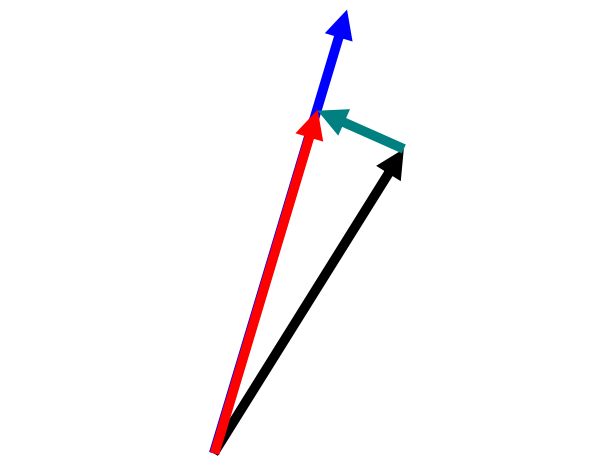
\includegraphics[width=0.45\linewidth]{chapter3_prove_3_8}
		\begin{minipage}[b]{0.5\linewidth}
			\itshape
			在这张示意图中,黑色线条表示当前时刻的$\vec{r}^f$,绿色线条表示在$\dif t$中由于$\mathcal{F}_{rotation}$的旋转导致的极径矢量改变,蓝色线条表示在$\dif t$中由于%$\mathcal{F}_{ratation}$和
			质点的平动导致的极径矢量改变。至于同时因旋转和平动导致的改变,由于是个二阶小量,这里并不画出。
			\vspace{1em}\quad
		\end{minipage}
		
		可以注意到,黑色线条旋转至红色线条产生的夹角为$-\vec{\omega}\Delta t$,且由于该角是个无穷小量,可以认为绿色线条与黑色线条正交,并且,我们还有绿色线条的长度为$r^f\omega\Delta t$。那么,绿色线条恰好可以表示为:
		\[{\color{green!50!black}\Delta\vec{r}}=(-\vec{\omega}\Delta t)\times \vec{r}^f\]
		至于蓝色线条,则可简单地通过平动速度得到:
		\[{\color{blue}\Delta\vec{r}}=\vec{v}_{/z}%-\vec{v}_{f/z})
		\Delta t\]
		求和即得$\Delta t$内质点在$\mathcal{F}_{rotation}$中极径矢量的变化量为
		\begin{align*}
			\Delta\vec{r}^f&={\color{green!50!black}\Delta\vec{r}}+{\color{blue}\Delta\vec{r}}\\
			&=(-\vec{\omega}\Delta t)\times \vec{r}^f+\vec{v}_{/z}-%\vec{v}_{f/z})
			\Delta t\\
			&=(-\vec{\omega}\times\vec{r}^f+\vec{v}_{/z}%-\vec{v}_{f/z}
			)\Delta t
		\end{align*}
		相除即得
		\[\vec{v}_{/z}^f=\dfrac{\Delta \vec{r}^f}{\Delta t}=-\vec{\omega}\times\vec{r}^f+\vec{v}_{/z}%-\vec{v}_{f/z}
		\]
		我们把上式变换形式:
		\begin{align*}
			(\dfrac{\dif\ }{\dif t})\vec{r}=(\dfrac{\mathrm{D}\ }{\mathrm{D} t}-\vec{\omega\times})\vec{r}
		\end{align*}
		
	\end{prove}
\end{comment}
\newcommand{\base}[1]{\hat{\vec{#1}}}
\begin{prove}[\itr{Frame Translation with Rotation}{考虑转动的参考系变换}*]
	这一次,我们采用坐标分解的观点思考问题。
	
	首先,考虑一个惯性系,并建立一个常规的空间直角坐标系$\mathcal{F}$,它的基为$\hat{\vec{i}},\hat{\vec{j}},\hat{\vec{k}}$,即为$x,y,z$轴方向的单位向量(单位向量没有量纲,长度为1)。那么,任取一个质点,它的位矢$\vec{P}$可以表示为\[
	\vec{P}=x\hat{\vec{i}}+y\hat{\vec{j}}+z\hat{\vec{k}}
	\]
	我们另建立一个拥有$x',y',z'$轴的,以角速度$\vec{\omega}$旋转的坐标系$\mathcal{F}'$,其中$z'$轴作为旋转轴与$z$轴平行。设该坐标系原点位矢$\vec{O'}$在原参考系中的表达式为$\vec{O}=x_0\hat{\vec{i}}+y_0\hat{\vec{j}}+z_0\hat{\vec{k}}$,那么在$\mathcal{F}'$中,设
	\[\vec{P}-\vec{O'}=\vec{P}'=x'\hat{\vec{i}'}+y'\hat{\vec{j}'}+z'\hat{\vec{k}'}\]
	如此,我们说,$\vec{P}$在$\mathcal{F}$中的坐标为$(x,y,z)$,在$\mathcal{F}'$中的坐标为$(x',y',z')$。
	
	接下来,我们考虑在不同坐标系中的速度。
	
	$\mathcal{F}$中的速度定义为\[\vec{v}=v_x\base{i}+v_y\base{j}+v_z\base{k}\]其中
	\[v_x=\dfrac{\dif x}{\dif t},v_y=\dfrac{\dif y}{\dif t},v_z=\dfrac{\dif z}{\dif t}\]
	于是
	\begin{align}
		\dfrac{\dif\vec{P}}{\dif t}&=\dfrac{\dif(x\hat{\vec{i}})}{\dif t}+\dfrac{\dif(y\hat{\vec{j}})}{\dif t}+\dfrac{\dif(z\hat{\vec{k}})}{\dif t}\\
		&=\dfrac{\dif x}{\dif t}\hat{\vec{i}}+\dfrac{\dif y}{\dif t}\hat{\vec{j}}+\dfrac{\dif z}{\dif t}\hat{\vec{k}}\\
		&=v_x\hat{\vec{i}}+v_y\hat{\vec{j}}+v_z\hat{\vec{k}}\\
		&=\vec{v}
	\end{align}
	其中由(3.2)到(3.3)的理由是该参考系的基$\hat{\vec{i}},\hat{\vec{j}},\hat{\vec{k}}$始终不变。
	
	同理,$\mathcal{F}'$中的速度定义为
	\[\vec{v}'=v_x'\base{i'}+v_y'\base{j'}+v_z'\base{k'}\]
	其中
	\[v_x'=\dfrac{\dif x'}{\dif t},v_y'=\dfrac{\dif y'}{\dif t},v_z'=\dfrac{\dif z'}{\dif t}\]
	\\[1ex]
	由$\vec{P}'=\vec{P}-\vec{O'}$,且$\vec{O}'$不变,知$\dfrac{\dif \vec{P'}}{\dif t}=\dfrac{\dif\vec{P}}{\dif t}=\vec{v}$。于是有
	\begin{align}
		\vec{v}&=\dfrac{\dif\vec{P}'}{\dif t}\\
		&=\dfrac{\dif(x'\hat{\vec{i}'})}{\dif t}+\dfrac{\dif(y'\hat{\vec{j}'})}{\dif t}+\dfrac{\dif(z'\hat{\vec{k}'})}{\dif t}\\
		&=\dfrac{\dif x'}{\dif t}\hat{\vec{i}'}+\dfrac{\dif\hat{\vec{i}'}}{\dif t}x'+\dfrac{\dif y'}{\dif t}\hat{\vec{j}'}+\dfrac{\dif\hat{\vec{j}'}}{\dif t}y'+\dfrac{\dif z'}{\dif t}\hat{\vec{k}'}+\dfrac{\dif\hat{\vec{k}'}}{\dif t}z'
	\end{align}
	注意到
	\[\dfrac{\dif\base{i'}}{\dif t}=\vec{\omega}\times\base{i'},\dfrac{\dif\base{j'}}{\dif t}=\vec{\omega}\times\base{j'}\]
	续(3.7)有
	\begin{align}
		\vec{v}&=v_x'\base{i'}+v_y'\base{j'}+v_z'\base{k'}+\vec{\omega}\times\base{i'}x'+\vec{\omega}\times\base{j'}y'\\
		&=\vec{v}'+\vec{\omega}\times\vec{r}'\qquad(\text{这里记}\vec{r}'=x'\base{i'}+y'\base{j'})
	\end{align}
	关于加速度,我们有类似的定义
	\[\left\{\begin{array}{c}
		\vec{a}=a_x\base{i}+a_y\base{j}+a_z\base{k}\\[1ex]
		a_x=\dfrac{\dif v_x}{\dif t},a_y=\dfrac{\dif v_y}{\dif t},a_z=\dfrac{\dif v_z)}{\dif t}
	\end{array}
	\right.\]
	\[\left\{\begin{array}{c}
		\vec{a}'=a_x'\base{i'}+a_y'\base{j}'+a_z'\base{k'}\\[1ex]
		a_x'=\dfrac{\dif v_x'}{\dif t},a_y'=\dfrac{\dif v_y'}{\dif t},a_z'=\dfrac{\dif v_z'}{\dif t}
	\end{array}
	\right.
	\]
	对(3.9)左右两侧同时对时间微分,有
	\begin{align}
		\mathrm{LHS}&=\dfrac{\dif\vec{v}}{\dif t}\\
		&=\dfrac{\dif v_x}{\dif t}\base{i}+\dfrac{\dif v_y}{\dif t}\base{j}+\dfrac{\dif v_z}{\dif t}\base{k}\\
		&=\vec{a}
	\end{align}
	\begin{align}
		\mathrm{RHS}&=\dfrac{\dif\vec{v}'}{\dif t}+\dfrac{\dif(\vec{\omega}\times\vec{r}')}{\dif t}\\
		&=\dfrac{\dif(v_x'\base{i}')}{\dif t}+\dfrac{\dif(v_y'\base{j}')}{\dif t}+\dfrac{\dif(v_z'\base{k}')}{\dif t}+\dfrac{\dif\vec{\omega}}{\dif t}\times\vec{r}'+\vec{\omega}\times\dfrac{\dif\vec{r}'}{\dif t}\\
		&=\vec{a}'+\vec{\omega}\times(v_x'\base{i'}+v_y'\base{j'})+\vec{\alpha}\times\vec{r}'+\vec{\omega}\times\dfrac{\dif\vec{r}'}{\dif t}
	\end{align}
	记$v_x'\base{i'}+v_y'\base{j'}=\vec{v}_{/z}'$,则续(3.15)有
	\begin{align}
		\mathrm{RHS}&=\vec{a}'+\vec{\omega}\times\vec{v}_{/z}'+\vec{\alpha}\times\vec{r}'+\vec{\omega}\times(\vec{v}_{/z}'+\vec{\omega}\times\vec{r}')\\
		&=\vec{a}'+2\vec{\omega}\times\vec{v}_{/z}'+\vec{\alpha}\times\vec{r}'-\omega^2\vec{r}'
	\end{align}
	这里注意到$\vec{\omega}\times\vec{v}_{/z}'=\vec{\omega}\times\vec{v}'$,因为$\vec{v}_z'$与$\vec{\omega}$平行。
	
	于是将左式与右式联立,得
	\[\vec{a}'=\vec{a}-2\vec{\omega}\times\vec{v}'-\vec{\alpha}\times\vec{r}'+\omega^2\vec{r}'\]
	其中(3.16)$\Rightarrow$(3.17)有关双重叉乘见\refleaftext{chapter3_double_cross_product}
	
	两侧同时乘以$m$,即得牛顿第二定律形式
	\[m\vec{a}'=m\vec{a}-2m\vec{\omega}\times\vec{v}'-m\vec{\alpha}\times\vec{r}'+m\omega^2\vec{r}'\]
	这意味着,如果希望牛顿运动定律在$\mathcal{F}'$中依然成立,我们需要对$\mathcal{F}'$中的物体添加三个假想力,分别是$-2m\vec{\omega}\times\vec{v}',\quad-m\vec{\alpha}\times\vec{r}',\quad m\omega^2\vec{r}'$。
	
	如果我们将条件简化,认为$\mathcal{F}'$没有角加速度,则有
	\[m\vec{a}'=m\vec{a}-2m\vec{\omega}\times\vec{v}'+m\omega^2\vec{r}'\]
	当$\mathcal{F}'$还拥有平动速度,平动加速度时,只需依照矢量叠加原理分析,再添上惯性力,牛顿第二定律就能继续保持成立。
\end{prove}
	
\chapter[流体力学]{\itr{Fluid Mechanics}{流体力学}}

	{\LARGE \centering \color{red}\itshape
		BLANK\\
		期待你的建设
		
	}
	%\input{../chapters/chapter5/chapter5_prove}
	\input{../chapters/chapter6/chapter6_prove}
 	\input{../chapters/chapter7/chapter7_prove}
	\apart{答案部分}
	\chapter[测量]{\itr{Measurement}{测量}}
\begin{solution}[\\The \itr{displacement}{位移} of a particle moving under \itr{uniform
		acceleration}{匀加速度} is some function of the \itr{elapsed time}{经历的时间} and
	the acceleration. Suppose we write this displacement
	$s=ka^mt^n$,where A is a \itr{dimensionless constant}{无量纲常数}. \\
	(1)Show by
	dimensional analysis that this expression is satisfied if
	$m = 1$ and $n = 2$. \\
	(2)Can this analysis give the value of A?]
	(1) 观察等式$s=ka^mt^n$,有:
	\begin{align*}
		\text{左式量纲}&=L\\
		\text{右式量纲}&=(\dfrac{L}{T^2})^m\cdot(T)^n=L^mT^{n-2m}
	\end{align*}
	联立两式即得
	\[m=1,n=2\]
	\par
	(2) 不能,量纲分析只是定性分析,无法解决值上的问题。
\end{solution}
	\chapter{}
	\chapter[转动动力学]{\itr{Rotation Dynamics}{转动动力学}}
\begin{solution}[{\large\color{plainred}Determine the Moment of Inertia of an Irregularly Shaped Object}\\
	This problem describes one experimental method of
	determining the moment of inertia of an irregularly
	shaped object such as the \itr{payload}{有效负载} for a satellite. \\
	The figure shows a mass $m$ \itr{suspended}{悬挂} by a \itr{cord}{绳子} \itr{wound}{被缠绕}
	around a spool of radius $r$, forming part of a \itr{turntable}{转台}
	supporting the object. When the mass is released from
	rest, it \itr{descends}{下降} through a distance $h$, acquiring a speed
	$\vec{v}$. Show that the moment of inertia $I$ of the equipment
	(including the turntable) is\quad$mr^2(\dfrac{2gh}{v^2}-1)$. ]
	\begin{center}
		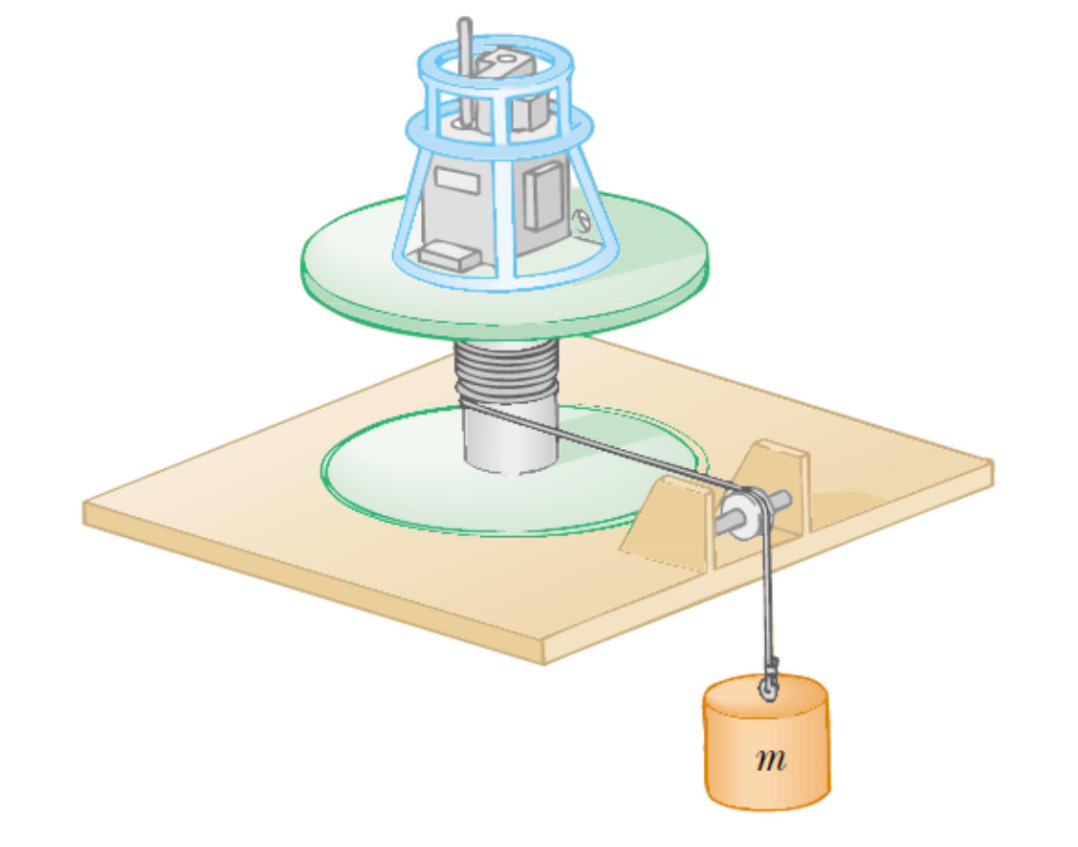
\includegraphics[width=0.6\textwidth]{chapter3_example_1}
	\end{center}
	
	这是一道基础的转动力学题目,一般的求解思路为:列力学方程---列运动方程---列关联方程---求解。
	
	设绳子的张力为$\vec{T}$,物体的转动惯量为$I$,有:
	\[\left\{
		\begin{array}{cc}
			\left.\begin{array}{c}
				Tr=I\alpha\\
				mg-T=ma
			\end{array}\right\}&\cdots\text{力学方程}\\
			v^2=2ah&\cdots\text{运动方程}\\
			a=r\alpha&\cdots\text{关联方程}
		\end{array}
		\right.\]
	联立求解即得\[I=mr^2(\dfrac{2gh}{v^2}-1)\]
\end{solution}
\begin{solution}[{\large\color{plainred}Rolling Items}\\
	Three objects of \itr{uniform density}{均匀的密度} --- a \itr{solid sphere}{实心球}, a \itr{solid
		cylinder}{实心圆柱}, and a \itr{hollow cylinder}{空心圆柱} --- are placed at the top of
	an \itr{incline}{斜坡}. \\
	If they all are released from rest
	at the same \itr{elevation}{高度} and roll without \itr{slipping}{滑动}, which object reaches the bottom first?
	]
	\begin{center}
		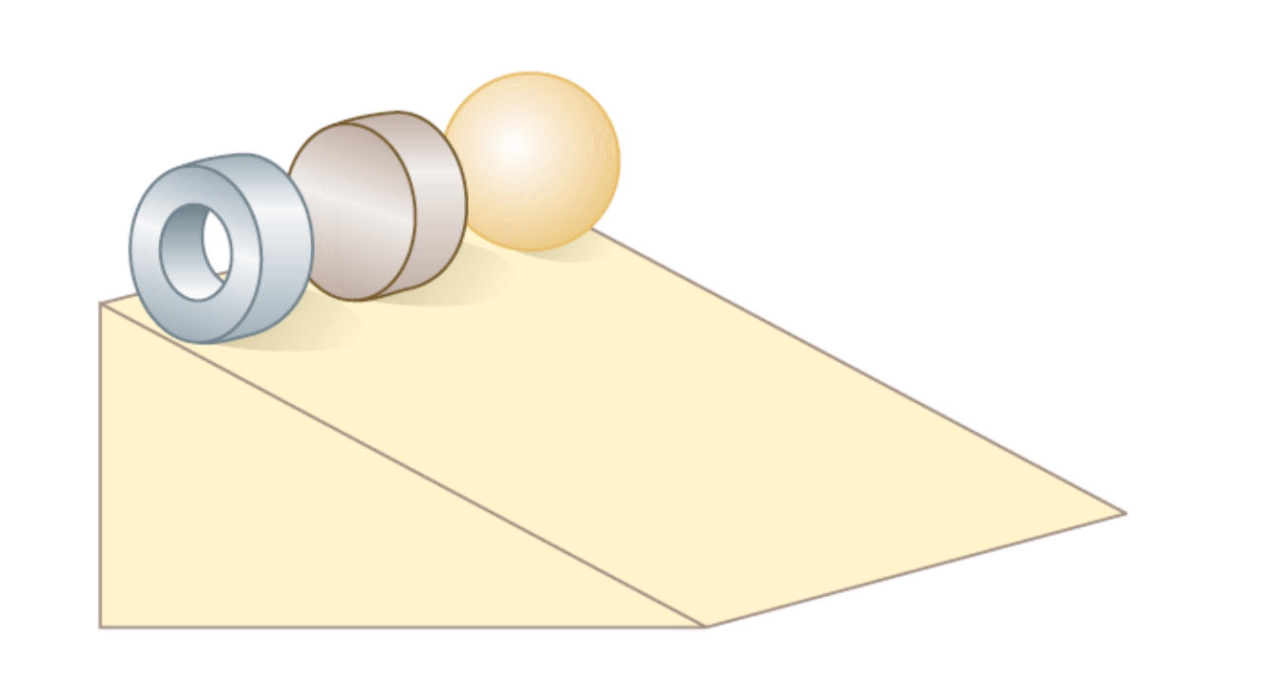
\includegraphics[width=0.6\textwidth]{chapter3_example_2}
	\end{center}
	
	本题是经典的纯滚动问题。所谓纯滚动,就是滚动体与接触面接触的点速度为$\vec{0}$(即旋转速度和质心速度相抵消)。
	%分析纯滚动时,我们往往以接触线为转动轴,以避免引入非惯性系,将问题复杂化。
	
	我们往往选择过质心的轴作为旋转轴,建立参考系。这是因为,即使这样建立的参考系是一个非惯性系,只要它不发生转动,那么,使用证明“均匀重力场中重力可以等效作用在质心”中用到的方法(\refleaftext{prove3.7}),就可以证明惯性力可以等效作用在质心。由于我们选择的是质心轴,惯性力产生的力矩恒为$0$,因此也就不会对转动的分析产生影响\footnote{很多解析都直接选择了一个非惯性质心系来分析转动,却并没有讲解惯性力可以忽略的原因。}。
	
	现在,让我们选择质心系分析问题\footnote{当然,过质心的轴有很多,但是大家应该能意会到选择了怎样的轴(对称性好的轴),就不再描述了}。
	
	若记球体$m_1$的转动惯量为$I_1$,实心圆柱$m_2$的转动惯量为$I_2$,空心圆柱$m_3$的转动惯量为$I_3$,斜面倾角为$\theta$,则有:
	\[\left\{
		\begin{array}{l}
			m_1a_1=m_1g\sin\theta-f_1\\
			m_2a_2=m_2g\sin\theta-f_2\\
			m_3a_3=m_3g\sin\theta-f_3\\
			 f_1r_1=I_1\alpha_1\\
			 f_2r_2=I_2\alpha_2\\
			 f_3r_3=I_3\alpha_3\\
			a_1=r_1\alpha_1\\
			a_2=r_2\alpha_2\\
			a_3=r_3\alpha_3
		\end{array}
	\right.\]
	于是解得
	\[\left\{
		\begin{array}{l}
			a_1=\dfrac{m_1r_1{}^2}{I_1+m_1r_1{}^2}g\sin\theta\\[2ex]
			a_2=\dfrac{m_2r_2{}^2}{I_2+m_2r_2{}^2}g\sin\theta\\[2ex]
			a_3=\dfrac{m_3r_3{}^2}{I_3+m_3r_3{}^2}g\sin\theta
		\end{array}
	\right.\]
	由常见物体的转动惯量(见\refleaftext{chapter3_moment_inertia2})知
	\begin{align*}
		I_1&=\dfrac{2}{5}m_1r_1{}^2\\
		I_2&=\dfrac{1}{2}m_2r_2{}^2\\
		I_3&=\dfrac{1}{2}m_3(r_{3(inner)}{}^2+r_3{}^2)
	\end{align*}
	易知
	\[a_1>a_2>a_3\]
	故实心球快于实心圆柱快于空心圆柱。
\end{solution}
%\refleaf*{law3.1}[-40ex]
%\refleaf*{chapter3_moment_inertia2}[-35.6ex]
\newpage
\begin{solution}[\En{\large Calculation of the Moment of Inertia}\\A rod's \itr{linear density}{线密度} is given by $\lambda=kx$, where $x$ represents the distance from the point to the rod's center. \\
	Given the length of the rod $l$, try to calculate the moment of inertia of the rod, given the rotation axis at:\\	
	(1) Center $O$ as the $y$ axis shows.\\
	(2) One end as the $y'$ axis shows.]
	\begin{center}
		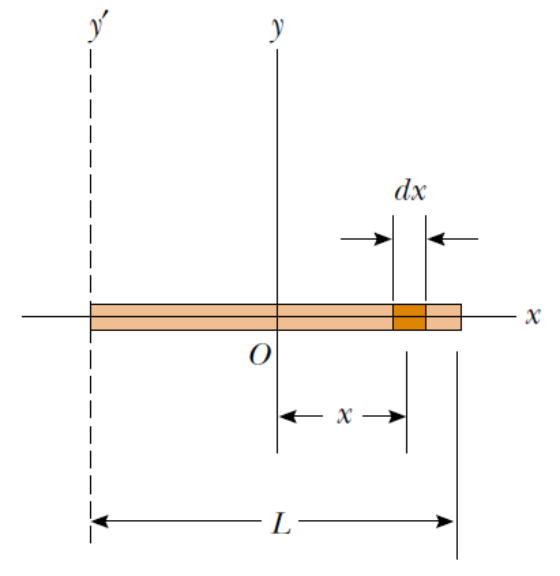
\includegraphics[width=0.5\textwidth]{chapter3_rod}
	\end{center}
	(1)由于$O$也是质心位置,不妨先求$I_{CM}$,再利用平行轴定理求解$I_{end}$。
	注意到
	\[\dif m=\lambda\dif x=k|x|\dif x\]
	于是
	\begin{align*}
		\int_{-\frac{L}{2}}^{\frac{L}{2}}(x^2)(k|x|)\dif x&=2\int_0^{\frac{L}{2}}kx^3\dif x\\
		&=2\left.(\dfrac{1}{4}kx^4)\right|_0^{\frac{L}{2}}\\
		&=\dfrac{1}{32}kL^4
	\end{align*}
	
	(2)欲用平行轴定理(\refleaftext{law3.1}),则需知晓棍子的质量。
	\begin{align*}
		m&=\int_{-\frac{L}{2}}^{\frac{L}{2}}k|x|\dif x\\
		&=2\int_0^{\frac{L}{2}}kx\dif x\\
		&=2\left.(\dfrac{1}{2}kx^2)\right|_0^{\frac{L}{2}}\\
		&=\dfrac{1}{4}kL^2
	\end{align*}
	故
	\[I_{end}=I_{CM}+m(\dfrac{L}{2})^2=\dfrac{3}{32}kL^4\]
\end{solution}
\begin{solution}[\En{\large Massive \itr{Pulley}{滑轮}}\\Consider two \itr{cylinders}{圆柱} having masses $m_1$
	and $m_2$, where $m_1 < m_2$, connected by a
	string passing over a pulley. The pulley
	has a radius $R$ and moment of inertia $I$
	about its axis of rotation. The string does
	not \itr{slip}{滑动} on the pulley, and the system
	is released from rest. Find the linear
	speeds of the cylinders after
	cylinder 2 \itr{descends}{下降} through a
	distance $h$, and the angular
	speed $\omega$ of the pulley at this time.]
	\begin{center}
		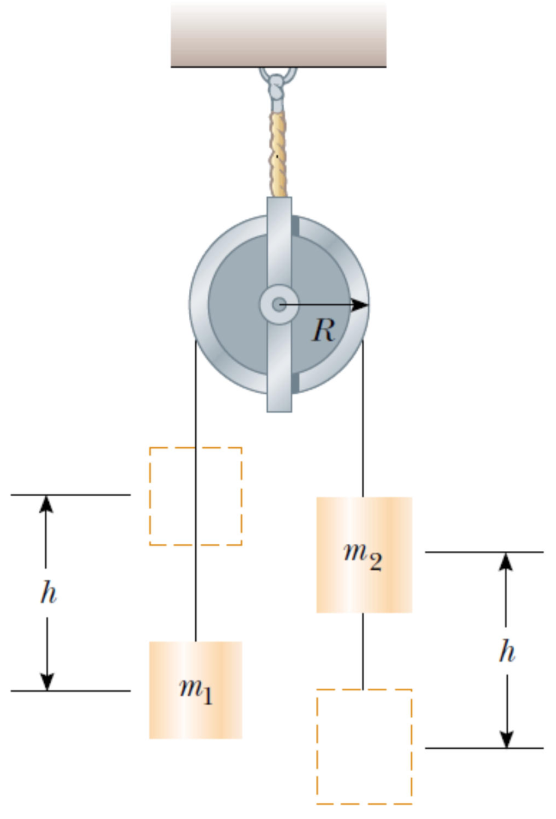
\includegraphics[width=0.3\textwidth]{chapter3_massive_pulley}
	\end{center}
	本题可从运动角度或能量角度考虑。\\
	法一:运动分析\\
	设左绳的张力为$T_1$,右绳的张力为$T_2$,则有
	\[\left\{\begin{array}{c}
		T_1-m_1g=m_1a\\
		T_2R-T_1R=I\alpha\\
		m_2g-T_2=m_2a\\
		a=R\alpha
	\end{array}\right.\]
	于是解得
	\[a=\dfrac{m_2-m_1}{m_1+m_2+\frac{I}{R^2}}g\]
	则
	\[v=\sqrt{2ah}=\sqrt{\dfrac{m_2-m_1}{m_1+m_2+\frac{I}{R^2}}2gh},\quad\omega=\sqrt{\dfrac{m_2-m_1}{(m_1+m_2)R^2+I}2gh}\]
	法二:能量分析\\
	系统机械能守恒,于是有
	\[\left\{\begin{array}{c}
		m_2gh=m_1gh+\dfrac{1}{2}m_1v^2+\dfrac{1}{2}m_2v^2+\dfrac{1}{2}I\omega^2\\
		v=R\omega
	\end{array}\right.\]
	亦可解得
	\[v=\sqrt{2ah}=\sqrt{\dfrac{m_2-m_1}{m_1+m_2+\frac{I}{R^2}}2gh},\quad\omega=\sqrt{\dfrac{m_2-m_1}{(m_1+m_2)R^2+I}2gh}\]
\end{solution}
\begin{solution}[\En{\large Object rotating on a string
		of changing length}\\Initially, the mass \itr{revolves}{转动} with a speed $v_1$ = 2.4 m/s in
		a circle of radius $R_1$ = 0.80 m.
		The string is then pulled slowly through the hole so
		that the radius is reduced to $R_2$ = 0.48 m. What is the
		speed, $v_2$, of the mass now?]
	\begin{center}
		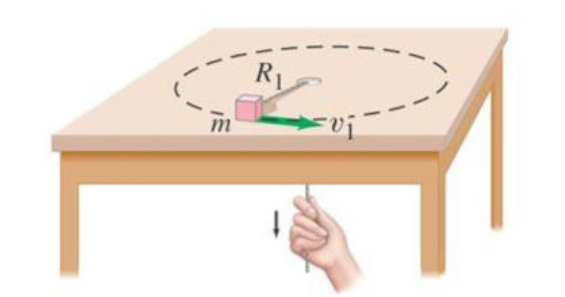
\includegraphics[width=0.7\textwidth]{chapter3_string}
	\end{center}
	本题考察角动量守恒。可以注意到,绳子对物块的力始终是径向的,对应的力矩始终为$\vec{0}$,因此,物块的角动量守恒。不妨就以洞为轴,有
	\[I_1\omega_1=I_2\omega_2\Rightarrow R_1{}^2\omega_1=R_2{}^2\omega_2\]
	代入$\omega_1=\dfrac{v_1}{R_1},\quad\omega_2=\dfrac{v_2}{R_2}$,即得
	\[v_1R_1=v_2R_2\]
	代入数据即得$v_2=4.0$m/s.
\end{solution}
\begin{solution}[\En{\large Rotation of a sliding rigid rod}\\Consider a rod with mass m and length L standing straight on the friction-less ground. When we
	release the rod, it will fall from the unstable \itr{equilibrium position}{平衡位置}\!.\\
	(a) Calculate the angular velocity of the rod, when it has an angle of $\theta$ with respect to the ground
	as illustrated in Figure 1.\\
	(b) What is the final angular velocity $\omega_1$ of the rod before it hits the ground?\\
	(c) If the same rod is leaning to a frictionless wall with an initial angle of α to the frictionless
	ground (see Figure 2), what is the final angular velocity $\omega_2$ of the rod before it hits the ground?\\
	{\em Note that there is a possibility that the right end of the rod leaves from the wall before the rod hits the ground.}]
	\begin{center}
		\begin{minipage}{0.45\textwidth}
			\centering
			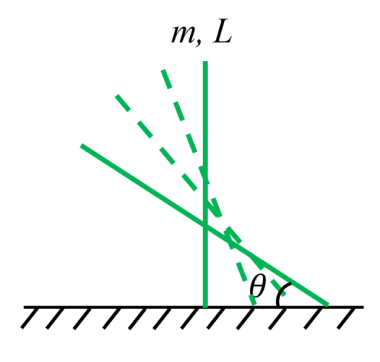
\includegraphics[width=\linewidth]{chapter3_rotating_rod_1}\\
			Figure 1
		\end{minipage}
		\quad
		\begin{minipage}{0.45\textwidth}
			\centering
			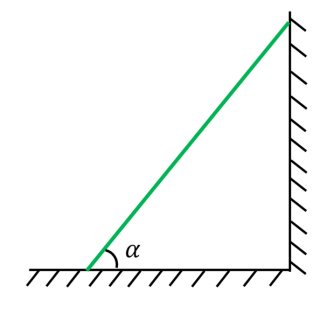
\includegraphics[width=\linewidth]{chapter3_rotating_rod_2}\\
			Figure 2
		\end{minipage}
	\end{center}
	本题主要考察转动中的能量守恒,以及对平动速度和角速度关系的分析。
	
	(a) 首先,由题意知不存在摩擦力,而支持力做功始终为零,所以以棍子为研究对象,有机械能守恒。又注意到,棍子在水平方向始终不受力,因此质心是在垂直下降。于是有
	\begin{equation}
		mg\dfrac{L}{2}-mg\dfrac{L}{2}\sin\theta=\dfrac{1}{2}mv_{CM}{}^2+\dfrac{1}{2}I\omega^2
	\end{equation}
	研究质心的运动,有
	\begin{align}
		v_{CM}&=\dfrac{\dif (\frac{L}{2}\sin\theta)}{\dif t}\\[1ex]
		&=\dfrac{L}{2}\dfrac{\dif\sin\theta}{\dif\theta}\dfrac{\dif\theta}{\dif t}\\[1ex]
		&=\dfrac{L}{2}\cos\theta\omega
	\end{align}
	将(3.4)代入(3.1)即得
	\begin{equation}
		\omega=2\sqrt{\dfrac{3g}{L}\dfrac{1-\sin\theta}{1+3\cos^2\theta}}
	\end{equation}
	(b) 即考虑(a)中的极限情况,将$\theta=0$代入(3.5)中即得
	\begin{equation}
		\omega_1=\sqrt{\dfrac{3g}{L}}
	\end{equation}
	(c) \begin{center}
		\begin{tikzpicture}[scale=2]
			\coordinate (O) at (0,0);  
			\coordinate (A) at (-1,0);  
			\coordinate (B) at (0,1.732); 
			\coordinate (D) at (-1.5,0);
			\coordinate (E) at (0,2.5); 
			\coordinate (BB) at (0,1.414);
			\coordinate (AA) at (-1.414,0);
			
			\draw [green](A) -- (B) ; 
			\draw [thick=3pt](D)--(O);
			\draw [thick=3pt](O)--(E);
			\draw [green,dashed](AA)--(BB);
			
			\coordinate (M) at ($(A)!0.5!(B)$);  
			\coordinate (N) at ($(AA)!0.5!(BB)$);
			
			\draw[dashed,plainred] (O) -- (M);  
			\draw[dashed,plainred] (O)--(N);
			\draw[dashed,yellow5] (0,0) circle[radius=1];
			
			\node[below left] at (A) {$A$};  
			\node[above right] at (B) {$B$};  
			\node[above right] at (BB) {$B'$};
			\node[below left] at(AA) {$A'$};
			\node[above left] at (M) {$C$};  
			\node[below left] at (O) {$O$};  
			\node[above right]at (A) {$\ \ \ \alpha$};
			\node[above left] at (N) {$C'$};
			\draw (-0.8,0) arc(0:60:0.2);
			\draw (-1.214,0) arc (0:45:0.2);
			\node[above right] at (AA) {$\ \ \ \,\theta$};
		\end{tikzpicture}  
	\end{center}
		
如图,先考虑棍未与墙壁脱离情形,注意到质心$C$到$O$的距离始终为$\dfrac{L}{2}$,因此确定质心的运动轨迹是一个圆。由$\angle COA=\angle CAO$,知$v_{CM}=\omega\dfrac{L}{2}$,即关系式。再由\\[1ex]“无摩擦力”,“支持力不做功”知棍子机械能守恒,于是可以列出守恒式:
		\begin{equation}
			mg(\dfrac{L}{2}\sin\alpha-\dfrac{L}{2}\sin\theta)=\dfrac{1}{2}mv_{CM}{}^2+\dfrac{1}{2}I\omega^2
		\end{equation}
由(3.7)可解得
\begin{equation}
	\omega=\sqrt{\dfrac{3g(\sin\alpha-\sin\theta)}{L}}
\end{equation}
接下来,我们考虑临界条件。当棍子脱离墙时,来自墙的支持力消失,也就是说,\textbf{质心在水平方向不再拥有加速度}。于是,$v_{CMx}$最大时,棍子将脱离墙。
\begin{align}
	v_{CMx}&=v_{CM}\sin\theta\\
	&=\omega\dfrac{L}{2}\sin\theta\\
	&=\dfrac{\sin\theta}{2}\sqrt{3gL(\sin\alpha-\sin\theta)}\\
	&=\sqrt{3gL}\cdot\sqrt{\dfrac{\sin\theta}{2}}\cdot\sqrt{\dfrac{\sin\theta}{2}}\cdot\sqrt{\sin\alpha-\sin\theta}\\
	&\le\dfrac{1}{3}\sin\alpha\sqrt{gL\sin\alpha}\quad(\text{当且仅当}\sin\theta=\dfrac{2}{3}\sin\alpha)
\end{align}
之后,在水平方向,质心的运动保持不变。由(3.4)知,当棍子即将落地时,有\begin{equation}
	v_{CMy}=\dfrac{L}{2}\omega_2
\end{equation}于是可以列守恒式
\begin{equation}
	mg\dfrac{L}{2}\sin\alpha=\dfrac{1}{2}m(v_{CMx}{}^2+v_{CMy}{}^2)+\dfrac{1}{2}I\omega_2{}^2
\end{equation}
将(3.14)代入(3.15)即得
\begin{equation}
	\omega_2=\sqrt{(9\sin\alpha-\sin^3\alpha)\dfrac{g}{3L}}
\end{equation}
\dove\ PS:这大概是本章考察的天花板了。
\end{solution}

	\chapter[流体力学]{\itr{Fluid Mechanics}{流体力学}}
\begin{solution}[\\A fluid is rotating at constant angular velocity $\omega$ about the central vertical axis of a cylindrical container.\\
    (a)Show that the \itr{variation}{变化} of pressure in the \itr{radial direction}{径向} is given by $\dfrac{\dif p}{\dif r}=\rho \omega^2 r$.\\
    (b)Take $p=p_c$ at the axis of rotation (r=0) and show that the pressure $p$ at any point $r$ is
    \[
        p=p_c+\dfrac{1}{2}\rho\omega^2 r^2
    \]
    (c)Show that the liquid surface is of \itr{paraboloidal}{抛物面的} form; that is, a vertical cross section of the surface is the curve $y=\dfrac{\omega^2 r^2}{2g}$]
    \begin{center}
    	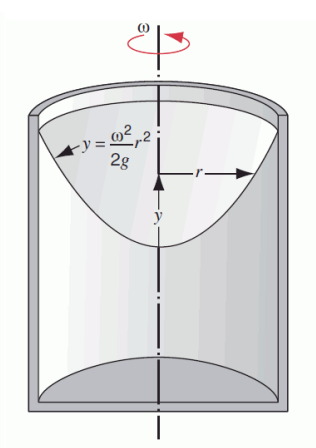
\includegraphics[width=0.45\textwidth]{chapter4_流体静力学}\\
    	\itshape 流体静力学
    \end{center}
    (a)取一段竖直方向的薄平面,设其截面积为A,沿半径方向的厚度为$\dif r$,深度为$h$。如下图所示:
    \begin{singlefigure}[A-4-1]{chapter4_E1_A1}[0.45]
    \end{singlefigure}

    可知水平方向的压强差为$\dif p=p_{r+\dif r}(h)-p_r(h)$,其中$p=p_0+\rho gh$。由受力关系结合匀速圆周运动可得:
        \[F=A\dif p=A\dif r \rho \omega^2 r\]
    整理得到(a)中的公式。
    
    (b)化简上式并积分:
        \[\int_{p_{h,0}}^{p_{h,r}}\dif p=\int_{0}^{r}\rho \omega^2 r\dif r\]

    得到:$p=p_0+\rho gh+\dfrac{\rho \omega^2 r^2}{2}$。其中前两项与半径无关,即为$p_c$,可得:
        \[p=p_c+\dfrac{1}{2}\rho \omega^2 r^2\]
        
    (c)液体表面的压强均为大气压强,将$p=p_0$、$p_c=p_0+\rho gh$代入(b)中得到的公式,得:
        \[\rho gh+\dfrac{1}{2}\rho \omega^2 r^2=0\]
    由于深度的坐标轴是向下的,我们以页面最低点处的水平方向为r轴,沿中心线竖直方向作为y轴,也就是调转一下坐标系。应用上述公式可知:
        \[y=\dfrac{\omega^2 r^2}{2g}\]
\end{solution}
\newpage
\begin{solution}[\\As shown in Figure 4-2, it is an \itr{air suction device}{空吸装置}. Given that the depth of the centerline of the \itr{catheter}{导管} below the liquid level in container $A$ is $h$, 
	the height difference between the liquid level in container $B$ and the centerline of the horizontal catheter is $h_b$, \itr{the cross-sectional area}{横截面积} at the \itr{nozzle}{喷嘴} $d$ is $S_d$, 
	and the cross-sectional area at the \itr{contraction section}{收缩段} $c$ is $S_c$. What are the conditions for the \itr{ratio}{比率} of $S_d$ to $S_c$ to occur for \itr{suction}{抽吸}?
    ]
    \begin{center}
    	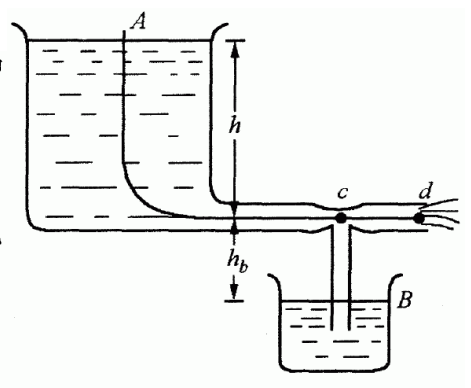
\includegraphics[width=0.65\textwidth]{chapter4_流体动力学}\\
    	\itshape 流体动力学
    \end{center}
    取一个流线Acd,对c、d两点应用伯努利公式可得:
        \[\dfrac{1}{2}\rho v_c^2+p_c=\dfrac{1}{2}\rho v_d^2+p_d\]
    其中d点的流速为$v_d=\sqrt{2gh}$,气压为大气压强$p_d=p_0$。且由于连续性原理,有:
        \[v_c S_c=v_d S_d\]
    因此c、d两点的压强差为:
        \[p_c-p_0=\rho gh(1-(\dfrac{S_d}{S_c})^2)\]
    而容器B液面的压强也是大气压强。发生空吸作用只要满足条件:
        \[p_c<p_0-\rho gh_b\]
    代入公式即可得到:
        \[\dfrac{S_d}{S_c}>\sqrt{1+(\dfrac{h_b}{h})}\]
\end{solution}
	%\input{../chapters/chapter5/chapter5_answer}
	\input{../chapters/chapter6/chapter6_answer}
 	\input{../chapters/chapter7/chapter7_answer}
\end{document}
